%Hauptdokument der Erstsemesterzeitschrift "Erste" der Fachgruppe Informatik
% TO DO:
% - Anpassen der Anrede: du
% - Rechtschreibkorrektur
% - Aktualisierung von Beiträgen
% - Recherche nach neuen Bildern
% - Rechteklärung mit den Profs wegen Fotos
% - 
\documentclass[]{papertex}
	\usepackage[utf8]{inputenc}
	\usepackage{graphicx}
	\usepackage{amssymb}
	\usepackage[T1]{fontenc}
	\usepackage{multicol}
	%\usepackage{hyperref}
	\usepackage[babel,german=quotes]{csquotes}

	\renewcommand{\familydefault}{\sfdefault}

	\clubpenalty = 10000
	\widowpenalty = 10000 
	\displaywidowpenalty = 10000

	% Trennregeln
	\hyphenation{
		AStA
		Mit-be-wohnerIn-nen
		Pro-fessorInnen
		erwischt
		viiieel
		y-Nummer
		Uniaccount
	}

\begin{document}
	\thispagestyle{empty}
	\clearpage
	\setcounter{page}{1}
	\tableofcontents
	
\section{Vorwort}
\label{vorwort}
	\begin{multicols}{2}
	\subsection*{Willkommen in der Informatik!}	

	Ein neues Semester hat begonnen und wieder strömen unzählige neue Gesichter auf den Campus um das Abenteuer Studium zu beginnen oder fortzusetzen. Da das nicht immer ganz einfach ist haben wir, die Fachgruppe Informatik für die Erstsemester unserer Fachrichtung einen kleinen Leitfaden zusammengestellt - die 1-te.

	Auf den folgenden Seiten werden wir hoffentlich einige der typischen Fragen beantworten, die einen am Anfang des Studiums quälen. Außerdem möchten wir natürlich uns, die Fachgruppe vorstellen (s. Seite \pageref{fachgruppe}) und eventuell noch die ein oder andere hilfreiche Information mitgeben. 

	\subsubsection*{Aufbau dieses Heftes}
		In der ersten Hälfte dieses Heftes sind wichtige
		Erklärungen zum Studienbeginn, dem Studiengang und der
		universitären Infrastruktur. Weitere Informationen zu
		uns und unserer Gremienarbeit, sowie weitere
		Informationen sind in der zweiten Hälfte.
\columnbreak
	\subsubsection*{Die Fachgruppe Online}
		Natürlich gibt es uns auch online - auf der Seite \url{http://fginfo.cs.tu-bs.de}. Beispielsweise stehen dort aktuelle Termine wie Spiele- oder Grillabende. Auch gibt es dort noch einmal die Inhalte dieses Heftes, samt den Aktualisierungen die erst nach dem Druck bekannt wurden. 

	\vspace*{0.5cm}

	Viel Spaß und Erfolg im  Studium wünscht  die\\
	\hspace*{2cm}Fachgruppe Informatik
	\end{multicols}
	\vspace{0.5cm}
	\begin{center} 
\includegraphics[totalheight=12cm]{bilder/XKCD/dorm_poster}
\end{center}

	\newpage
	\section{Die ersten Tage}
		%\subsection{Termine}
\label{termine}
	\begin{multicols}{2}
	Gerade in der Anfangszeit des Studiums gibt es eine Menge zu tun. Damit du
	nicht das Wichtigste verpasst, haben wir die ersten Termine kompakt für
	dich zusammengefasst. Die meisten davon bieten die Gelegenheit Fragen zu
	stellen und nebenbei gleich ein paar nette Kommilitonen kennen zu lernen.

	Falls du  es dir nicht schon gedacht habt: Die Spalten B und M geben an,
	ob der Termin für Bachelor- oder Masterstudenten gedacht
        ist. Falls du den eigentlichen Termin verpasst, kannst du
        stattdessen auch zum anderen erscheinen. Es besteht die Chance, dass sich einige Orte
	und Zeiten
	nach Drucklegung noch Ändern.  Bei den mit ,,*'' markierten Zeiten und
	Orten ist das besonders wahrscheinlich. Schaue deshalb bitte vorher
	nochmal im Blog \url{http://fginfo.cs.tu-bs.de/} nach, ob die Angaben
	noch aktuell sind. Dort kannst du übrigens auch den Kalender digital abonnieren.
	Du findset die Termine auch online unter \url{http://tinyurl.com/3ltuzbb}.
	Wenn du einen Dienst, ein Handy oder eine Software nutzt, die das iCalender-Format unterstützt
	kannst du die Termine auch von dort aus einbinden und hast sie somit im Blick. 
	Dazu gehören z.\,B. iPhone, Android, Google Calendar, Outlook\,\dots. Eine Liste 
	von ca. 60 Programmen findest du unter 	\url{http://tinyurl.com/yns84t}
	\end{multicols}

	\begin{tabular}{|l|l|p{6.7cm}|c|c|c|}
	\hline \textbf{Datum} 		& \textbf{Uhrzeit} 	& \textbf{Veranstaltung}						& \textbf{Ort} 	& \textbf{B}	& \textbf{M} 	\\
	\hline 26.09. – 30.09.		& 1. Tag: 10:00	 	& Vorkurs Informatik							& PK 2.1		& B				& 				\\
		   17.10. – 21.10.		& 					& 												& 				& 				&    			\\
	\hline Mo, 24.10. 			& 09:00 – 10:00		& Begrüßung	durch den Präsidenten				& Stadion		& B				& M				\\ 
	\hline 						& 10:00 – 12:00	 	& Infobörse										& Altgebäude	& B				& M				\\
	\hline   					& 10:00 – 11:00	 	& Begrüßung (M) \newline durch den Studiendekan	& IZ 160		& 				& M				\\
	\hline 						& 14:00 – 15:00	 	& Begrüßung (B) \newline durch den Studiendekan	& PK 11.3		& B				& 				\\
	\hline 						& 15:00 – 16:30		& Erste Vorlesung ,,Programmieren 1''			& SN 19.1		& B 			&				\\
	\hline Di, 25.10.			& 10:00 – 11:45 	& Erstsemester-Frühstück 						& IZ Plaza 		& B 			& M 			\\ 
	\hline 						& 12:00 – 13:30 * 	& FG-Einführung und \newline Stundenplan-Bauen 	& ??? * 		& B 			&  				\\%& ??? * & B &\\
	\hline 						& 12:00 – 13:30 * 	& FG-Einführung und \newline Stundenplan-Bauen 	& IZ 160 * 		& 				& M				\\
	\hline 						& 13:30 – 15:00 	& Rundgang mit den  Tutorengruppen 				& IZ 160 		& B 			& M				\\
	\hline Mi, 26.10.			& 10:00 – 17:00		& Studium Generale								& Altgebäude	& B				& M 			\\
	\hline Do, 03.11. 			& 19:00 			& Kneipentour der Fachgruppe 					& IZ 150 		& B 			& M				\\
	\hline Mi, 09.11.	 		& 19:00 			& Spieleabend der Fachgruppe 					& vor  150 		& B 			& M				\\
	\hline
	\end{tabular} 
%
%	\begin{multicols}{2}
%	Ihr findet die Termine auch online unter \url{http://tinyurl.com/3ltuzbb}.
%	Falls ihr einen Dienst, ein Handy oder eine Software nutzt, die das iCalender-Format unterstützt
%	könnt ihr die Termine auch von dort aus einbinden und habt sie somit im Blick. 
%	Dazu gehören z.\,B. iPhone, Android, Google Calendar, Outlook\,\dots. Eine Liste 
%	von ca. 60 Programmen findet ihr unter 
%	\url{http://tinyurl.com/yns84t}
%	\end{multicols}
 Raus da auf Miniausgabe und in Erstie-Infozettel enthalten, muss dann nciht aktualisiert werden
		% !TEX root = ../../1-te.tex

\subsection{Checkliste}
\label{checkliste}
	Hier wird zusammengefasst, was du in den ersten Tagen des Studiums unbedingt erledigen solltest. Wenn du die ToDos auf der Checkliste nach Erledigung abhakst, verlierst du nicht den Überblick und vergisst nichts.
	
\vspace*{0.5cm}
% !TEX root = ../../1-te.tex

\begin{center}
\begin{tabular}{|p{3mm}|l|p{8cm}|c|c|}
\hline \checkmark 
       & \textbf{Todo}             & \textbf{Zu erledigen bis}                                  & \textbf{Seite}               & \textbf{Muss?} \\ 
\hline & BAföG beantragen          & Spätestens Ende \iftoggle{winter}{Oktober}{April}          & \pageref{todobafoeg}         & optional \\ 
\hline & Wohnsitz ummelden         & 1 Woche nach Umzug                                         & \pageref{todoummelden}       & ja \\
\hline & Mailinglisten             & So früh wie möglich                                        & \pageref{mailinglisten}      & ja \\ 
\hline & Studiengrobplanung        & Vor dem Stundenplan bauen                                  & \pageref{grob}               & ja \\
\hline & Auflagen klären           & So früh wie möglich, final: Ende 2. Semester               & \pageref{auflagen}           & nur Master \\ 
\hline & Persönlicher Stundenplan  & Siehe Terminzettel der Fachgruppe                          & \pageref{masterstundenplan}  & ja \\ 
\hline & Prüfungsbogen             & Spätestens \iftoggle{winter}{Dezember}{Mai}                & \pageref{todoanmeldung}      & ja \\ 
\hline & Prüfungsanmeldung         & 12.12.2017 - 11.01.2018, schriftlich oder online           & \pageref{todoanmeldung}      & ja \\ 
\hline & Blog abonnieren           & So früh wie möglich                                        & \pageref{fachgruppe}         & ja \\ 
\hline & Prüfungsordnung lesen     & Zu den ersten Klausuren                                    & \pageref{po}                 & ja \\ 
\hline & TUcard validieren         & Zu Beginn und zu jedem neuen Semester                      & \pageref{tucard}             & ja \\
\hline & Bibliotheksausweis        & Vor der ersten Buchausleihe                                & \pageref{todobib}            & optional \\
\hline & Stud.IP-Nachrichten weiterleiten  & Wenn man nichts verpassen möchte         & \pageref{tumails}            & optional \\
\hline
\end{tabular} 
\end{center}
\tocheck{4}{Exakte Daten Anmeldewoche einfügen, s.\url{https://www.tu-braunschweig.de/fk1/service/informatik/pa}}

\begin{multicols}{2}

\subsubsection{BAföG}
	\label{todobafoeg}

	Wer Studierendenförderung nach dem Bundesausbildungsförderungsgesetz (BAföG) beantragen möchte, sollte sich am besten gründlich informieren. Sehr zu empfehlen ist da: \\
	\verUrl{4}{https://www.xn--bafg-7qa.de/}
 
	Förderungsanträge gibt es zum Download oder in Papierform im EG des Amtes für Ausbildungsförderung in der Wilhelmstraße 1. Wenn du BAföG beantragen möchtest, stelle den Antrag so früh wie möglich, denn es wird nicht rückwirkend gezahlt.

	Zum Anfang des Semester ist mit längeren Wartezeiten zu rechnen, im Notfall kannst du beim AStA-Sozialreferat ein kurzfristiges, zinsloses Darlehen beantragen, um den ersten Monat zu überbrücken. Das Darlehen ist auf 450 Euro begrenzt und muss spätestens nach drei Monaten zurückgezahlt werden. Mehr Informationen findest du auf der Seite des Sozialreferats: \verUrl{4}{https://www.asta.tu-braunschweig.de/referate/sozialreferat/}


\subsubsection{Ummelden}
	\label{todoummelden}

	Wer neu nach Braunschweig gezogen ist, muss sich innerhalb einer Woche beim Einwohnermeldeamt anmelden. Wenn ihr die Frist verpasst, drohen theoretisch Strafen, aber praktisch sieht es da nicht so streng aus. Wenn man Braunschweig als Erstwohnsitz wählt, bekommt man (ein Jahr später) eine einmalige Zuzugsprämie von 100 Euro (Immatrikulationsbescheinigung nicht vergessen). Alternativ kann man Braunschweig auch als Zweitwohnsitz wählen.

\subsubsection{Prüfungsanmeldung}
	\label{todoanmeldung}

	Du musst dich für alle Prüfungen, an denen du teilnehmen willst, vorher beim Prüfungsamt anmelden. Die Fristen sind relativ früh im Semester. Die Termine werden im Laufe des Semesters veröffentlicht (Seiten des P-Amtes (\verUrl{3}{https://www.tu-braunschweig.de/fk1/service/informatik/pa}), Mailingliste). Prüfungen können im Prüfungsanmeldezeitraum schriftlich im Prüfungsamt oder online über das QIS-Portal angemeldet werden.
	Vor deiner ersten Prüfungsanmeldung musst du außerdem ein Datenblatt ausfüllen. Es empfiehlt sich, das bereits vor der Anmeldewoche zu machen, weil die Schlangen dann nicht so lang sind.

	Für die Online-Anmeldung benötigst du eine TAN-Liste, die du dir vorher im Prüfungsamt organisieren musst.

	Unter folgendem Link findest du außerdem alle Prüfungstermine für die Informatik:
	\verUrl{3}{https://www.tu-braunschweig.de/fk1/service/informatik/pa}

\subsubsection{TUcard}
	\label{tucard}
	
	Alle Studierenden der TU erhaten den elektronische Studierendenausweis TUcard, die auch als Bibliotheksausweis und Mensakarte genutzt werden kann.

	Damit die Karte gültig ist, muss sie zu Beginn und zu jedem neuen Semester validiert werden. Das bedeutet, dass der Thermostreifen auf der Karte in einem Validierungsdrucker mit den aktuellen Daten beschrieben wird.

	Das Börsenguthaben der Karte, beispielsweise zum Bezahlen in der Mensa, kann an Börsenaufwertern (auch denen, die sich bereits in den Mensen befinden) aufgeladen werden.

	Zum Drucken kann Guthaben der Karte auf ein Druckkonto umgebucht werden. Dies geschieht an den Druckkontenumbuchern.

	Weitere Informationen zur TUcard findest du unter: \verUrl{3}{https://www.tu-braunschweig.de/studium/imstudium/tucard}

\subsubsection{Uni-Bibliothek}
	\label{todobib}

	Um Bücher in der Uni-Bibliothek ausleihen zu können, brauchst du einen Ausweis. Dieser ist in deiner TUcard integriert. Diesen kannst du an einem der Terminals in der Bibliothek, oder online beantragen und am Schalter freischalten. Je nachdem, ob du zu Beginn schon Bücher brauchst, kannst du die Karte auch später aktivieren.

	In der Bibliothek stehen außerdem Kopierer bereit, die du nutzen kannst. Einen davon kannst du mit Kleingeld befüllen, kompfortabler geht es aber mit einer Kopierkarte. Die bekommst du für ein paar Euro direkt in der Bibliothek. Zu Semesterbeginn gibt es oft noch Einführungskurse in die Bibliotheksbenutzung. Ob du deinen Bibliotheksausweis vor oder nach diesem Kurs aktivierst, ist egal.
	
\end{multicols}

	\newpage
	\section{Studienplan(ung) für jeden}
		\label{studienplan}
		\subsection{Verantwortung}
	\textit{Große Macht bringt große Verantwortung mit sich!}, sagte schon Ben Parker, der Onkel von Spiderman. Das heißt für dich: Du hast die Macht und die Verantwortung über deinen Studienfortgang. Das beginnt bei der Entscheidung, überhaupt zu studieren, die Wahl des Faches und der Universität und erstreckt sich über die Wahl, welche Fächer du hörst und wann du das tust, bis hin zur Einflussnahme auf den gesamten Studiengang.

	Es besteht aber auch die Möglichkeit diese Verantwortung abzugeben. Es gibt einen Studienplan, der dir vorschlägt, wie du deine Fächer wählen und anordnen kannst, um in Regelstudienzeit fertig zu werden. Für den Bachelor sieht dieser Plan sehr konkret aus, für den Master ist er abstrakter gehalten, aber deckt immer noch nur partiell die Wahlmöglichkeiten ab. Das kann und soll er auch nicht -- es handelt sich um zwei von unendlich vielen Möglichkeiten, zum Studienabschluss zu kommen. % Verantwortung
		\subsection{Zwei Studiengänge unter einem Hut}
	Seit der Bologna-Reform gibt es an der TU Braunschweig zwei Studiengänge - \textit{Bachelor und Master}. Viele Informationen über das Studium betreffen beide, deshalb ist diese Zeitung für alle Erstsemester. Nach der allgemeinen Einleitung folgen die speziellen Abschnitte für Bachelor- (ab S. \pageref{bachelor}) und Master-Ersties (ab Seite \pageref{master}).

\subsubsection{Herden, Rudel und Einzelgänger}
	Bevor es in die Untiefen der Prüfungsordnungen und formalen Anforderungen geht, ein paar Worte zu einem sozialen Phänomen. Der recht feste Stundenplan im Bachelor-Studium sorgt dafür, dass man dort in der Regel mit vielen Mitstudierenden zusammensitzt, die in der gleichen Situation sind wie man selbst: Neu hier und mit den gleichen Fragen und Sorgen. Und ist ein Block zu Ende, so zieht man gemeinsam zum nächsten Raum, wo man mit praktisch der gleichen Gruppe das nächste Fach abgrast. Eine typische Herde also.

	Im Master ist das grundlegend anders. Jeder hört andere Vorlesungen, und in den \emph{Mastervorlesungen} tummeln sich nicht nur Masterstudierende, sondern auch Bachelor- und Diplom- oder gar fachverwandte Studierende, wie z.B. Wirtschaftsinformatik. Da kann es eine ganze Weile dauern, bis man weiß, wer auch im Masterstudium ist und gegebenfalls auch noch im gleichen Jahrgang. Selbst dann haben diese Leute ihren Bachelor hier oder dort, in diesem oder jenem Fach an einer Uni oder FH gemacht. Vielleicht haben die neben dir zuvor ganz andere Dinge gelernt, vielleicht sind sie hier um sich auf etwas komplett anderes zu spezialisieren als du.

	Keine Frage: Diese Mischung macht es spannender, bunter und vielseitiger, aber auf jeden Fall auch schwieriger. Wir können hier kaum Tipps geben, wie man als Neuling und eventuell unfreiwillige/r Einzelgänger/in ein kleines Rudel findet oder bildet. Weder wir noch dieses Heft könnten all das ersetzen, was eine Gruppe von Gleichgesinnten mit gleichen Problemen und Interessen könnte. Aber wir wissen, dass man in den ersten Tagen und Wochen viele Fragen hat. Gerade als Master hat man oft nur wenige Mitstudierende an der Seite, die die gleichen Fragen und/oder die passenden Antworten haben. Deshalb dieses Heft.

	Um deine Mitstudierenden schneller kennenzulernen, gibt es unter anderem die vielfältigen Angebote der Fachgruppe (Spieleabende, Kneipentouren, Grillen, etc.) - siehe \url{http://fginfo.cs.tu-bs.de/}
  % Bachelor und Master (Herden und Rudel)
		\subsection{Die Prüfungsordnung}
\label{po}
	An einer Universität gibt es tausende Regeln und Ordnungen. Die wichtigste ist die Prüfungsordnung: Sie enthält Antworten auf 95\% aller Fragen, die im Studium auftreten - nicht nur wenn es um die eigentlichen Prüfungen geht. Die genaue Bezeichnung lautet \emph{Besonderer Teil der Prüfungsordnung für den (Bachelor-/Master-)studiengang Informatik der Technischen Universität Braunschweig}. Und da sie weder besonders lang, noch kompliziert geschrieben ist, sollte jeder Student sie einmal überfliegen.

	Außerdem gibt es noch die APO, die Allgemeine Prüfungsordnung. Sie gilt uniweit für alle Studiengänge, doch die beiden BPOs überschreiben die meisten APO-Regelungen.

	Wenn du es noch nicht getan hast, lade dir deine aktuelle Prüfungsordnung am besten von \url{http://www.tu-braunschweig.de/fk1/service/informatik/dokumente} herunter. 


   % Prüfungsordnung
		% !TEX root = ../../1-te.tex

\subsection{Module und Co.}
	Um deinen Abschluss zu bekommen, musst du eine vordefinierte Menge von Modulen abdecken. Ein Modul besteht aus verschiedenen Bestandteilen.

\subsubsection{Vorlesung, Übung, etc.}
	\paragraph*{Vorlesung}
	Vorlesungen werden vor allen Studis abgehalten und befassen sich in erster Linie mit der theoretischen Herleitung des Stoffes. Solltest du in der Vorlesung einmal etwas nicht verstehen, so ist das nicht so tragisch. Vorlesungen an der Uni unterscheiden sich stark vom Unterricht an der Schule. Gehe nicht davon aus, Vorlesungsinhalte direkt zu verstehen. Plane eine gewisse Nachbearbeitungszeit für die Vorlesungen ein. In einer Vorlesung ist wegen der großen Teilnehmerzahl normalerweise kein Dialog mit dem oder der Vortragenden möglich. Aufgetretene Fragen können und sollten am besten direkt nach der Vorlesung oder sonst in einer Sprechstunde mit der oder dem Lehrenden geklärt werden.
	
	\paragraph*{Große Übung}
	Ergänzend gibt es die großen Übungen, auch Saalübungen genannt. Diese finden, wie die Vorlesung, vor dem gesamten Auditorium statt und sollen das erworbene, theoretische Wissen vertiefen und vor allem auch praktische, klausurbezogene Anwendungen aufzeigen. Die große Übung wird normalerweise von einer Mitarbeiterin oder einem Mitarbeiter gehalten. Sie sind bei  fachlichen Fragen kompetente Ansprechpartner/innen und meistens auch sehr hilfsbereit. Da sie  üblicherweise die Klausuren entwerfen, kann man bei genauem Hinhören in den großen Übungen oder im privaten Gespräch mit ihnen einiges über die Prüfung erfahren.

	\paragraph*{Kleine Übung, Seminargruppe}
	Als erstes eine Warnung: Kleine Übungen tauchen im Stundenplan nicht immer auf und werden leider nur in einigen Fächern angeboten. Der Begriff Seminargruppe ist synonym zu verstehen.
	
	In kleinen Übungen soll man selbst Aufgaben lösen. Dies geschieht unter Anleitung der HiWis (Hilfswissenschaftler/innen), welche meist Studierende höheren Semesters sind. Für die kleinen Übungen werden die Studis in etwa 20- bis 30-köpfige Gruppen aufgeteilt. Hierbei ist darauf zu achten, rechtzeitig zum Termin der Gruppeneinteilung zu erscheinen, um diese Veranstaltungen möglichst günstig im Stundenplan positionieren zu können. Der Termin wird meistens in der ersten Vorlesung bzw. großen Übung bekannt gegeben oder steht auf der jeweiligen Institutsseite. Aufgrund der geringen Teilnehmerzahlen ist in kleinen Übungen der Dialog mit der oder dem Vortragenden möglich und sinnvoll. Bei guten HiWis kann man in den kleinen Übungen all die Wissenslücken auffüllen, die nach Vorlesung und großer Übung offen sind.
	
	\paragraph*{Klausur}
	Klausuren sind schriftliche Prüfungen und finden in nahezu allen Pflichtfächern im Bachelor statt. Man kann sich noch bis 12:00 Uhr des vorherigen Werktags von einer schriftlichen Prüfung abmelden, online sogar bis 23:59 Uhr. Nach Bekanntgabe des Ergebnisses (im Regelfall nach 2-4 Wochen) gibt es meistens eine Einsicht. Die sollte auf jeden Fall besucht werden. Zum einen, weil ab und an Punkte übersehen werden und sich so die Note verbessern kann, aber auch der Lerneffekt ist nicht zu unterschätzen: Ist man durchgefallen, oder hat unerwartet schlecht abgeschnitten, so kann man dort dann erfahren, woran es gehapert hat und dies als Erkenntnisgewinn für das nächste Mal mitnehmen.

	\paragraph*{Mündliche Prüfungen}
	Mündliche Prüfungen gibt es in zwei Fällen: Als Prüfung anstelle einer Klausur, meistens in Fächern mit recht wenig Studierenden, wie in vielen Wahlpflicht- und Masterfächern. 
	%Im Bachelor sind hingegen nahezu alle Prüfungen schriftlich, laut Prüfungsordnung sind aber drei mündliche Prüfungen abzulegen. \\
	Der andere Fall ist die mündliche Nachprüfung: Sollte man dreimal durch eine Prüfung durchgefallen sein, kann man erst exmatrikuliert werden, wenn man zuvor eine sogenannte Ergänzungsprüfung abgelegt hat. Ein reines Bestehen reicht aus um weiterstudieren zu dürfen.\\
	Bei regulären mündlichen Prüfungen (also \emph{keine} Nachprüfung) kann man sich bis eine Woche vor dem Prüfungstermin abmelden.

	\xkcd{width=0.9\columnwidth}{compiling}

	\subsubsection{Seminar}
	Außerdem musst du sowohl im Bachelor als auch im Master ein so genanntes Seminar einbringen, das ist eine Ausarbeitung zu einem Thema, die meist aus einem Vortrag und einer mehrseitigen schriftlichen Arbeit besteht. Anders als für alle anderen Modularten muss man sich für das Seminar inklusive Themenwahl schon im Voraus anmelden. Die angebotenen Seminare finden sich auf den jeweiligen Institutswebseiten, die Anmeldung läuft über StudIP und die Institutsseiten. Da die Anzahl der Plätze in jedem Seminar begrenzt ist, solltest du ab Semster-Ende die Institutsseiten im Blick behalten und dich so früh wie möglich anmelden.

	Prinzipiell kannst du dir, wie bei den meisten Modulen, aussuchen, in welchem Semester du das Seminar einbringst. Viele orientieren sich aber an den Musterstudienplänen, weswegen die Seminare im Wintersemester oft überbucht, und im Sommersemester frei sind. Wenn du also ein Thema abbekommen möchtest, dass dir auch wirklich gefällt, solltest du darüber nachdenken, das Seminar ins Sommersemester zu verlegen.

	\subsubsection{Schlüsselqualifikationen / Mathe-Wahl\-pflicht}
	\tocheck{4}{Beschreibungen für BA und MA aktuell nach BPO?}
	Hier können überfachliche Veranstaltungen aus dem Schlüsselqualifikations-Pool eingebracht werden. Da dies ca. 100 angebotene Verstanstaltungen pro Semester sind, findest du sie nicht im Modulhandbuch oder im Informatik-Studenplan, sondern im QIS\footnote{\verUrl{4}{https://vorlesungen.tu-bs.de/qisserver/rds?state=wtree&search=1&trex=step&root120172=168835|172301&P.vx=kurz}}.
	 Zu beachten ist, dass man dabei nur Fächer belegen darf, die nicht aus dem eigenen Nebenfach stammen. Man kann also z.B. mit dem Nebenfach Mathe nicht Schlüsselqualifikationen der Mathematik belegen.
	 Daneben ist es möglich Veranstaltungen der \textit{Trainings handlungsbezogener Kompetenzen des Lehrstuhls für Arbeits"~, Organisations- und Sozialpsychologie} einzubringen\footnote{\verUrl{4}{https://www.tu-braunschweig.de/psychologie/abt/aos/studiumlehre/hbk}} oder des Sprachzentrums (siehe unten).
	Außerdem können vier Credits im Rahmen des \textit{SCOUT-Programm des Instituts für Arbeits"~, Organisations- und Sozialpsychologie} eingebracht werden. Hier werden internationale Studierende von dir als SCOUT ein Semester lang begleitet, um ihnen die Integration in den deutschen Unialltag zu erleichtern\footnote{\verUrl{4}{https://www.tu-braunschweig.de/scout}}. Soweit die Regelungen für beide Studiengänge, nun die spezifischen:

	\paragraph*{Schlüsselqualifikationen im Bachelor}
	Im Bachelor musst du fünf Credits in Schlüsselqualifikationen belegen, die du dir nahezu beliebig aussuchen darfst. Das Modul besteht aus mehreren unbenoteten Studienleistungen. Dies gilt auch dann, wenn du einen benoteten Schein bekommst.\\
	Außerdem musst du zehn Credits im Wahlpflichtbereich Mathematik erbringen. Die Auswahl besteht zur Zeit aus drei Fächern, eins im Winter und zwei im Sommer. Die beiden Wahlpflichtfächer Mathe gehen benotet ein.

	\paragraph*{Schlüsselqualifikationen im Master}
	Im Master kannst du acht bis zehn Credits als Schlüsselqualifikation belegen. Es gibt ansonsten nur einen Unterschied zur Bachelorregelung: Sofern du nicht gerade Mathe als Nebenfach belegst, kannst du dort auch Mathewahlpflichtfächer einbringen. Der Master hat sonst keinen Mathewahlpflichtbereich. Auch im Master besteht der Schlüsselqualifikationenblock aus unbenoteten Studienleistungen.

	\subsubsection{Sprachenzentrum}
	Am Sprachenzentrum der Uni kannst du verschiedene Sprachkurse belegen, die auch als Schlüsselqualifikationen zählen (maximal 8 Credits). Auf den Seiten des Sprachenzentrums (\verUrl{4}{https://www.tu-braunschweig.de/sprachenzentrum}) findest du alle angebotenen Kurse.

	\textbf{Wichtig:} Die Anmeldung für Sprachkurse beginnt bereits in den Semesterferien. Um Plätze zu bekommen, solltest du dich also so früh wie möglich anmelden. Vor der Teilnahme an ausgewählten Sprachkursen musst du zunächst einen Einstufungstest absolvieren. Die Termine und weitere Infos findest du hier: \verUrl{4}{https://www.tu-braunschweig.de/sprachenzentrum/sprachen/einstufungstests}\\
	Da bei einigen Kursen die Nachfrage sehr hoch ist, solltest du den Test möglichst bereits vor dem Anmeldungszeitraum (beginnt etwa 2 Wochen vor Vorlesungsbeginn) ablegen.

	\vspace{.5cm}
	\xkcd{width=0.9\columnwidth}{good_code}

	\subsubsection{Praktikum}
	Teilweise werden auf Vorlesungen aufbauende Praktika angeboten, die das erworbene Wissen praktisch vertiefen sollen. Der Ablauf sieht so aus, dass man bestimmte Aufgaben lösen und die Lösung abgeben muss. Anschließend sind die Ergebnise einem Übungsleiter vorzuführen und zu erklären. Es kann sich dabei um einzelne Teilaufgaben oder ein großes Softwareprojekt handeln, ähnlich dem SEP oder Teamprojekt. Im Regelfall handelt es sich bei Praktika um unbenotete Studienleistungen.

Es werden folgende	Arten von Praktika unterschieden:
	
	\begin{itemize}
		\item Es gibt Veranstaltungen, bei denen die Teilnahme am Praktikum verpflichtend ist, um den Schein zur Vorlesung zu bekommen. 
		\item Es gibt freiwillige Praktika als Alternative oder Ergänzung zur Vorlesung.
		\item Außerdem gibt es Prakika, bei denen man sich aussuchen kann, ob man sie als Teil einer Vorlesung (so genannte Supermodule) oder als eigenes Modul belegen möchte.
	\end{itemize}

\noindent	Die Menge der Praktika, die du in das Studium einbringst, wird u.a. dadurch beschränkt, wie viele unbenotete Studienleistungen du einbringen darfst, bzw. umgekehrt darüber, wie viele benotete Leistungen erwartet werden.


	\tocheck{4}{Beschreibungen aktuell nach BPO?}

	\subsubsection*{SEP (Software-Entwicklungs-Praktikum)}
	Eine Sonderform des Praktikums ist das SEP im Bachelor. Es wird üblicherweise im 4. Semester (Studienbeginn WS) oder 5. Semester (Studienbeginn SS) absolviert. Von normalen Praktika unterscheidet es sich dadurch, dass es verpflichtend ist. Es geht darum, im Team das \textbf{gelernte Wissen} aus den Vorlesungen \emph{Programmieren 1+2}, sowie \emph{Software Engeneering 1} anzuwenden, indem man ein Softwareprojekt (Entwicklung und Dokumentation) umsetzt. Das SEP ist eine unbenotete Studienleistung.

	\subsubsection*{Teamprojekt}
	Ebenfalls ein spezielles Praktikum ist das Teamprojekt. Es verfolgt eine ähnliche Zielsetzung wie das SEP, mit dem Unterschied, dass es weniger formale Vorgaben gibt und man sich selbst ein Thema suchen kann. Dazu empfiehlt es sich, rechtzeitig auf den Webseiten der Institute nachzuschauen und sich eine Gruppe zu suchen. Wie das SEP ist auch das Teamprojekt eine Studienleistung.

	\subsubsection{Projektarbeit im Master}
	Für den Master kommt noch die Projektarbeit hinzu. Dies ist eine
	freiwillige Prüfungsleistungsleistung, die aus einem eigenständig
	bearbeiteten Projekt mit schriftlicher Ausarbeitung besteht. Das Modul umfasst 15 Credits.

	\subsubsection{Abschlussarbeit}
	Die Abschlussarbeit sind 12 Credits im Bachelor und 30 Credits im Master. Dabei geht es darum, dass im Studium erworbene Wissen an einer gegebenen Aufgabenstellung anzuwenden und  die Ergebnisse in einer schriftliche Ausarbeitung festzuhalten. Wie beim Teamprojekt gilt auch hier, dass die Institute oft Themen vorschlagen.  Man kann auch ein eigenes Thema vorschlagen, wenn es ins Forschungsprofil des Institus passt. \textbf{Wichtig:} Bevor du die Abschlussarbeit anmelden kannst, musst du bestimmte Vorraussetzungen erfüllen:

	\begin{itemize}
		\item Bachelorarbeit: Sämtliche Pflichtfächer (Grundlagen der Informatik, Mathematik und Informatik der Systeme).
		\item Masterarbeit: Module im Umfang von 75 Credits müssen vor Anmeldung absolviert worden sein.
	\end{itemize}

%%% Local Variables: 
%%% mode: latex
%%% TeX-master: "../../1-te_ws"
%%% End: 
  % Module und Co.
		\subsection{Grobplanung zuerst}
\label{grob}
	Keine Sorge, deine \textit{Studiengrobplanung} ist ein abstraktes Konzept, du wirst sie nirgends aufschreiben und einreichen müssen, du kannst also große Teile davon so oft ändern wie du möchtest. Aber Vorsicht: Zum einen studiert es sich besser, wenn man von Anfang an weiß, wo es hin geht, zum anderen gibt es gewisse Entscheidungen, die man später nicht mehr ändern kann, wie z.B. das Nebenfach.
	%bla raus! (joke)
	%Aber dazu später mehr\ldots

\subsubsection{Wie viele Credit Points?}
	Standardmäßig sind 30 Credit Points pro Semester vorgesehen - so hat man nach 6 Semestern den Bachelor und nach weiteren 4 den Master in der Tasche. Man ist dann aber auch zeitlich sehr ausgelastet, und für Urlaub, Familie und Nebenjob bleibt nicht unbedingt Zeit. Wenn man im Master außerdem mit Zulassungsauflagen gesegnet ist, sind dies bis zu 15 weitere Credit Points, die man irgendwie auf die ersten beiden Semester aufteilen muss. Deshalb ist es hilfreich sich am Anfang des Studiums zu überlegen, wann man wie viele und ggf. sogar welche Module man belegen will.

	Ein weitere Frage am Anfang des Studiums ist die Finanzierung:
	BAFöG-Höchstförderungsdauer, Langzeitstudiengebühren, sowie das
	Ende von Kindergeld, Kindesunterhalt und Famlienversicherung bei
	der Krankenkasse können problematisch sein. Hiwi-Jobs,
	Studienkredite und Stipendien können helfen, aber vielleicht
	wieder Zeit fressen. 

	Was auch immer du nun denkst, wie viele CP du im kommenden Semester belegen möchte, plane vielleicht ein paar Reserve-Punkte ein, also zusätzliche Fächer, die du belegst. Du kannst dann immernoch im laufenden Semester Vorlesungen abbrechen, wenn es doch nicht so spannend ist wie zuerst gedacht (natürlich keine Pflichtveranstaltungen). Durchfallen ist weder eine Schande noch ein großes Problem, da es dir die Prüfungsordnung erlaubt, bis zu drei Fächer, bei denen du im 1. Versuch durchgefallen bist, so abzuwählen als hättest du sie nie belegt. Dennoch sollte man es vielleicht mit den Reservefächern nicht übertreiben.

\subsubsection{Nebenfach und Studienrichtung}
\label{nebenfach}
	Im Bachelor musst du, im Master kannst du ein Nebenfach wählen. Die Nebenfach-Enscheidung (ob und welches) will gut überlegt sein, denn der Wechsel ist nur unter sehr speziellen Bedingungen möglich, wenn man erstmal die erste Prüfung geschrieben hat.
 
	Die Studienrichtung ist  optional, aber im Gegensatz zum Nebenfach geht man damit keinerlei Verpflichtung ein. Am Ende des Studiums wird einfach geschaut, ob man 50 (Bachelor) oder 70 (Master) Credit Points in einem artverwanden Bereich erreicht hat und bekommt dann auf Wunsch ein Sonderprädikat aufs Zeugnis. Aber Vorsicht: manche Studienrichtungen erfordern außerdem noch, das man eine gewisse Untermenge von Seminar, Projektarbeit und Abschlussarbeit, sowie eine Mindestanzahl von Praktika im entsprechenden Bereich absolviert hat. Informiere dich also rechtzeitig! Im schlimmsten Fall kann einem aber nur passieren, dass man sich zwar in einer Richtung spezialisiert hat, darüber aber keinen expliziten Nachweis auf dem Zeugnis erhält.

	Beide Entscheidungen (Nebenfach, Studienrichtung) musst du nicht im ersten Semester treffen, sondern kannst dich auch später (aber am besten nicht zu spät) spezialisieren. Um dir dabei zu helfen, sammelt der Fachgruppenrat Berichte zu den Nebenfächern unter \url{http://fginfo.cs.tu-bs.de/} $\rightarrow$ Studium $\rightarrow$ Nebenfächer.

\subsubsection{Welche Fächer gibt es?}
	Die Liste der Fächer ist groß und ständig im Wandel. Offiziell festgelegt sind sie im Modulhandbuch (MHB). Unter \url{https://vorlesungen.tu-bs.de} findest du mit ein bisschen Suchen eine Übersicht über alle Fächer. Diese Fächer kannst du als Informatikstudierender belegen - aber nicht alle werden jedes Semester angeboten.

\subsubsection{Der generelle Stundenplan}
	Unter \url{http://theo.iti.cs.tu-bs.de/STP/stundenplan.php} findest du den aktuellen Plan. Dort sind die meisten Veranstaltungen der Informatikmodule eingetragen, allerdings ohne die Nebenfächer und den Schlüsselqualifikations-Pool. Der Stundenplan enthält sowohl Bachelor- als auch Masterfächer. Also musst du für jedes Fach, was du hier findest, erstmal verifizieren, ob du die Punkte überhaupt einbringen kannst. Wie du dir vielleicht schon denken kannst, wird dein persönlicher Stundenplan eine Untermenge dieses Mammut-Plans, erweitert um ein paar Veranstaltungen die hier nicht stehen.

	Wenn etwas darauf hindeutet, dass eine bestimmte Vorlesung im Semester angeboten wird, aber im Stundenplan nicht auftaucht, dann hilft eine Suche auf den Institutsseiten, und wenn selbst das nicht hilft, eine Mail an den oder die verantwortliche/n Lehrende/n. Das gleiche gilt, wenn irgendwas komisch wirkt, z.B. wenn im Stundenplan zu einem Fach 5 Übungstermine und kein Vorlesungstermin stehen.

\subsubsection{Auslandsaufenthalt}
	Über Auslandssemester solltest du dich ebenfalls so früh wie möglich mit dem \emph{International Office} (\url{http://tu-braunschweig.de/international}) in Verbindung setzen.

\subsubsection{Mentor/in und Beratungsgespräche}
	Laut Studienordnung bekommst du auch eine/n Mentor/in zugewiesen - das ist ein/e Professor/in aus der Informatik. Sie/Er soll dich bei Entscheidungen zum Studium im persönlichen Gespräch beraten. Gerade wenn du weißt, dass du dich spezialisieren möchtest, oder wenn du zumindest mit dem Gedanken spielst, solltest du eine/n Mentor/in haben, der aus der jeweiligen Fachrichtung kommt. Wird dir zu Beginn jemand völlig fachfremdes zugewiesen, dann kannst du recht formlos darum bitten, diesen zu wechseln. Gespräche mit der/dem Mentor/in sind weder verpflichtend noch planmäßig vorgesehen, sondern liegen in deiner eigenen Verantwortung.

Es gibt  noch weitere Ansprechpartner/innen für verschiedenste Anlässe. Die wichtigsten haben wir für dich unter  \url{http://fginfo.cs.tu-bs.de/} $\rightarrow$ Kontakt $\rightarrow$ Ansprechpartner zusammengefasst.
  % Grobplanung
	\newpage
	\section{Spezielles im Bachelor}
		\label{bachelor}
		% !TEX root = ../../1-te.tex

\subsection{Deine Veranstaltungen im ersten Bachelor-Semester}
	Um dir einen kleinen Vorgeschmack auf die Themen zu geben, die dich im ersten Semester beschäftigen könnten, gibt es hier einen Überblick:

	\nottoggle{winter}{Je nach deinen Vorkenntnissen kann es auch sinnvoll sein, andere Veranstaltungen (wie z.B. Technische Informatik oder Computernetze) zu belegen. Bevor du dich dazu entscheidest, solltest du dich aber auf jeden Fall durch uns beraten lassen.}{}

\tocheck{7}{Vorlesungsbeschreibungen mit Empfehlungen abgeleichen}
\tocheck{7}{Prüfen, dass Dozenten und Infos noch aktuell sind}

\iftoggle{winter}{
	% !TEX root = ../../../1-te.tex

\subsubsection{Algorithmen und Datenstrukturen}
	\textit{Prof. S\'andor Fekete}
	Diese Vorlesung vermittelt Programmiersprachenunabhängige Algorithmen und Konzepte wie Bäume, Listen oder Stacks. Wer nicht weiß, was sich hinter diesen Begriffen verbirgt, sollte auf keinen Fall die Übungen verpassen.
	\subsubsection{Programmieren 1}
	\textit{Dr. Werner Struckmann}
	Programmiert wird hier fast ausschließlich in Java. Wer keine oder nur wenig Erfahrungen mit Java gemacht hat, sollte unbedingt die kleinen Übungen bearbeiten.
	In Programmieren 1 (jährlich im Wintersemester) geht es um grundlegende Konzepte der Programmierung am Beispiel von Java. Darauf aufbauend wird in Programmieren 2 (jährlich im 	Sommersemester) die Implementierung von Algorithmen und Datenstrukturen geübt. 
	\xkcd{width=.9\columnwidth}{su_doku}
	% !TEX root = ../../../1-te.tex

\subsubsection{Diskrete Mathematik}
	\textit{Prof. Arnfried Kemnitz und PD JP Bode}
	Diskrete Mathematik handelt von allem, was mit ganzen Zahlen zu tun hat: Fibbonacci-Zahlen, Primzahlen, Modulorechnung, usw. Es werden die wichtigsten Mathemaischen Grundlagen vermittelt, unter anderem in Logik, Kombinatorik, Zahlentheorie und Algebra. Die kleinen Übungen sind hier eine sehr gute Vorbereitung auf die Hausaufgaben und die Klausur.
	% !TEX root = ../../../1-te.tex

\subsubsection{Lineare Algebra}
	\textit{Dr. Wolfgang Marten}
	Hier geht es um Vektoren und Matrizen, sowie ein wenig Gruppentheorie. Die Übungen sind zwar nicht immer einfach, geben aber einen sehr guten Ausblick auf die Klausur.	
	\subsubsection{Theoretische Informatik 1}
	\textit{Dr. Jürgen Koslowski}
	Hier geht es um formale Sprachen und Automatentheorie. Klingt theoretisch und mathelastig? Ist es auch. Nicht gleich aufgeben, wenn man in der Vorlesung nicht mitkommt, die kleinen Übungen helfen beim Verständnis und bei der Klausurvorbereitung. Sie ist regulär für das dritte Semester vorgesehen, wer es sich zutraut kann sie aber schon im ersten hören und sich damit den Stundenplan im dritten Semester ein wenig freihalten. 
	% !TEX root = ../../../1-te.tex

\subsubsection{Mathewahlpflicht}
%	\textit{N.N.} 
Ihr müsst insgesamt zwei Module zu je fünf Credits
	im Mathe-Wahlpflichtbereich einbringen. Dabei wird eine Vorlesung im Wintersemester und zwei
	Vorlesungen im Sommersemester angeboten:

	
	\begin{description} 
		\item[Algebra für Informatiker] \emph{(SoSe)} Hier gehts um grundlegende
		algebraische Strukturen (Mengen, Gruppen, Monide etc). Diese sind insbesondere für die
		theoretische Informatik von großer Bedeutung.
		\item[Einführung in die Stochastik für Informatiker] \emph{(SoSe)} Die
		Vorlesung behandelt die Grundlagen der
		Wahrscheinlichkeitstheorie (Laplace-Experimente,
		Erwartungswerte, Zufallsvariablen etc.). 
		\item[Einführung in die Numerik für Informatiker] \emph{(WiSe)} Hier werden Verfahren zum Lösen numerischer Probleme behandelt. 
%	 \item[Statistische Verfahren für Informatiker] Hier geht
%	es um statistische Probleme und wie man sie lösen kann.
%	Achtung: Die Vorlesung baut auf  ,,Einführung in
%	die Stochastik'' auf und setzt deren Inhalte voraus! Sie wird jedoch derzeit nicht angeboten.
	\end{description}

	Bei der Auswahl geht ihr am Besten so vor, dass ihr euch erstmal
	in alle gerade angebotenen reinsetzt und dann die behaltet, mit der ihr besser
	klarkommt. Generell gilt aber bei mathematischen Vorlesungen: Es
	gibt im Allgemeinen kein aktuelles Skript, wer nichts verpassen
	will, muss in der Vorlesung mitschreiben. Auch können die
	Hausaufgaben gerne mal umfangreicher werden, bereiten aber dafür
	sehr gut auf die Klausur vor. Dranbleiben und sich nicht
	entmutigen lassen ist alles :)
}{
	% !TEX root = ../../../1-te.tex

\subsubsection{Einführung in die Logik}
	\textit{Prof. Koslowski}
	Die Vorlesung behandelt die Grundlagen der formalen Logik, mit einen starken Fokus auf Aussagen- und Prädikatenlogik. Die Hausaufgaben sind dabei teilweise sehr zeitaufwändig, aber dafür eine gute Klausurvorbereitung. Dabei ist das Skript sehr hilfreich.
	% !TEX root = ../../../1-te.tex

\subsubsection{Analysis}
	\textit{Dr. Wolfgang Marten}
	Hier geht es um Differential- und Integralrechnung, sowie Grenzwerte. Die Übungen sind zwar nicht immer einfach, geben aber einen sehr guten Ausblick auf die Klausur. Die Übungsaufgaben sollte man umbedingt machen, wenn man vorhat die Klausur zu bestehen.
	\subsubsection{Programmieren 1}
	\textit{Dr. Werner Struckmann}
	Programmiert wird hier fast ausschließlich in Java. Wer keine oder nur wenig Erfahrungen mit Java gemacht hat, sollte unbedingt die kleinen Übungen bearbeiten.
	In Programmieren 1 (jährlich im Wintersemester) geht es um grundlegende Konzepte der Programmierung am Beispiel von Java. Darauf aufbauend wird in Programmieren 2 (jährlich im 	Sommersemester) die Implementierung von Algorithmen und Datenstrukturen geübt. 
	\xkcd{width=.9\columnwidth}{su_doku}
	\subsubsection{Algorithmen und Datenstrukturen 2}
	\textit{Prof. S\'andor Fekete}
	\todo[inline]{AuD2}
	%Diese Vorlesung vermittelt Programmiersprachenunabhängige Algorithmen und Konzepte wie Bäume, Listen oder Stacks. Wer nicht weiß, was sich hinter diesen Begriffen verbirgt, sollte auf keinen Fall die Übungen verpassen.
	% !TEX root = ../../../1-te.tex

\subsubsection{Computernetze}
	\textit{Prof. Dr.-Ing. Lars Wolf}
	In Computernetze geht es darum wie Computer miteinander kommunizieren und wie das Internet funktinoiert. Du lernst welche Protokolle im WWW zum Einsatz kommen, wozu man sie braucht und wie sie funktionieren. 
	% !TEX root = ../../../1-te.tex

\subsubsection{Technische Informatik}
	\textit{Prof. Rolf Ernst}
	Die Vorlesung zu Technischen Informatik orientiert sich
	weitgehend an dem Lehrbuch \enquote{Logic and Computer Design
	Fundamentals – 4th edition} von M. Mano und Ch. Kime, welches
	gleichzeitig als Skript gilt. Das Buch findet man in
	ausreichender Anzahl in der UB. Die kleinen Übungen sind als
	Klausurvorbereitung zu empfehlen, ersetzen aber nicht das eigene
	Nacharbeiten. 
	% !TEX root = ../../../1-te.tex

\subsubsection{Mathewahlpflicht}
%	\textit{N.N.} 
Ihr müsst insgesamt zwei Module zu je fünf Credits
	im Mathe-Wahlpflichtbereich einbringen. Dabei wird eine Vorlesung im Wintersemester und zwei
	Vorlesungen im Sommersemester angeboten:

	
	\begin{description} 
		\item[Algebra für Informatiker] \emph{(SoSe)} Hier gehts um grundlegende
		algebraische Strukturen (Mengen, Gruppen, Monide etc). Diese sind insbesondere für die
		theoretische Informatik von großer Bedeutung.
		\item[Einführung in die Stochastik für Informatiker] \emph{(SoSe)} Die
		Vorlesung behandelt die Grundlagen der
		Wahrscheinlichkeitstheorie (Laplace-Experimente,
		Erwartungswerte, Zufallsvariablen etc.). 
		\item[Einführung in die Numerik für Informatiker] \emph{(WiSe)} Hier werden Verfahren zum Lösen numerischer Probleme behandelt. 
%	 \item[Statistische Verfahren für Informatiker] Hier geht
%	es um statistische Probleme und wie man sie lösen kann.
%	Achtung: Die Vorlesung baut auf  ,,Einführung in
%	die Stochastik'' auf und setzt deren Inhalte voraus! Sie wird jedoch derzeit nicht angeboten.
	\end{description}

	Bei der Auswahl geht ihr am Besten so vor, dass ihr euch erstmal
	in alle gerade angebotenen reinsetzt und dann die behaltet, mit der ihr besser
	klarkommt. Generell gilt aber bei mathematischen Vorlesungen: Es
	gibt im Allgemeinen kein aktuelles Skript, wer nichts verpassen
	will, muss in der Vorlesung mitschreiben. Auch können die
	Hausaufgaben gerne mal umfangreicher werden, bereiten aber dafür
	sehr gut auf die Klausur vor. Dranbleiben und sich nicht
	entmutigen lassen ist alles :)
}

		\subsection{Interview mit PD Dr. Bode}
	Privatdozent Dr. Bode leitet die große Übung zur Vorlesung \emph{Diskrete Mathematik für Informatiker}, die jährlich im Wintersemester stattfindet. Er hat sich freundlicherweise für ein Interview zur Verfügung gestellt.
	\begin{description}
		\item[Was und wo haben Sie studiert?] 

		Ich habe hier an der Technischen Universität Mathematik mit Nebenfach Informatik studiert. Neben dem Diplom in Mathe habe ich dazu noch das Vordiplom in Informatik gemacht.
		\item[Welchen Bezug haben Sie als Mathematiker zu Informatik?] 

		Für mich sind Computer in erster Linie ein Werkzeug, um bestimmte mathematische Probleme zu lösen. Im Studium habe ich dazu hauptsächlich Vorlesungen aus der theoretischen Informatik gehört. Daneben habe ich als studentische Hilfskraft die Vorlesungen\emph{Theoretische Informatik 1/2} betreut.
		\item[Worum geht es in der Veranstaltung \emph{Diskrete Mathematik für Informatiker}?] 

		Sie behandelt wichtige Grundlagen, die die Studierenden später brauchen werden. Inhaltlich geht es zunächst um allgemeine Grundlagen, bevor wir uns etwas Kombinatorik, Zahlentheorie und Algebra angucken.
		\item[Welche Rolle spielen dabei die Übungen?] 

		Nun, die Übungen sind eine Ergänzung zur Vorlesung, die beim Verständnis helfen sollen. Dazu sind sie eine gute Vorbereitung für die Klausur. Dies klappt aber nur bei aktiver Mitarbeit der Studierenden. Man sollte sich die Aufgaben schon vorher mal angeguckt haben, sonst bringt das nichts.\footnote{Anmerkung des Interviewers: Das kann ich aus eigener Erfahrung bestätigen, auch wenn man dabei noch nichts versteht :)} Die Meisten verhalten sich leider am Anfang sehr passiv.
		\item[Was können Sie den Studierenden für die ersten Semester mit auf den Weg geben?] 

		Sie sollten  nicht alles glauben, was man ihnen erzählt. Vorletztes Jahr gab es das Gerücht, dass unsere 1. große Übung ausfällt, da es ja noch keine Vorlesung gab. Dem war nicht so, wir haben da die Übungseinteilung gemacht. Da weniger anwesend waren, gab es am Ende nicht so viele Übungen, wie man eigentlich gebraucht hätte. Im Zweifelsfall gilt die Webseite zur Übung \verUrl{0}{http://www.mathematik.tu-bs.de/jpbode/dm/}. Dort werden auch die Übungsblätter veröffentlich.\\ Neben diesen speziellen Ratschlag noch einen Allgemeinen: Niemand wird dafür umgebracht, Fragen zu stellen. Wenn also etwas unklar ist, nur Mut!
		\item[Vielen Dank für das Interview!] 

		Bitte sehr. Zum Abschluss möchte ich allen Erstsemestern noch viel Spaß und Erfolg im Studium wünschen.
	\end{description}
	%comic

		\subsection{Studienplan}
\label{bach_studienplan}
Wie ihr wahrscheinlich bereits in eurem Stundenplan festgestellt habt, müsst ihr im ersten Semester fünf Pflichtveranstaltungen hören.
Doch die Bezeichnung Pflichtverantstaltung sagt bloß aus, dass ihr die Veranstaltung \emph{irgendwann} einmal hören müsst, um euren Bachelor abschließen zu können.
Die zeitliche Abfolge der Veranstaltungen dürft ihr aber selbst festlegen.
Der von Frau Sehnert bereit gestellte Musterstudienplan (s. nächste Seite) bietet hier eine gute Orientierungsmöglcihkeit.
Ihr müsst euch aber nicht daran halten. Niemand zwingt euch eine Veranstaltung zu hören oder hält euch davon ab.
Ihr könnt euch eigentlich in jede Vorlesung setzen, auch ohne hinterher an der Prüfung teilnehmen zu müssen - allerdings gibts dann auch keine Punkte dafür.
Hier bieten sich zum Beispiel Module aus dem Wahlplichtbereich Informatik an, die eventuell nur alle 2 Jahre angeboten werden und über mehrere Semester gehen.
Bei den (Pflicht-)Modulen der Informatik müsst ihr jedoch beachten, dass einige Module auf anderen aufbauen.
Zum Beispiel sollten Programmierengrundlagen in den ersten zwei Semestern erarbeitet werden und mit Theoretische Informatik II werdet ihr euch schwer tun, wenn ihr TheoInf I nicht gehört habt.

Damit sich euer Studium nicht unnötig verlängert, solltet ihr aber darauf achten, in jedem Semester 30 Leistungspunkte zu erwerben. 


% Wie ihr wahrscheinlich bereits in eurem Stundenplan festgestellt habt,
% müsst ihr im ersten Semester drei "`Pflichtveranstaltungen'' hören.  
% Doch die Bezeichnung Pflichtverantstaltung sagt bloß aus, dass ihr die Veranstaltung \emph{irgendwann} einmal hören müsst, um euren Bachelor abschließen zu können.
% Die zeitliche Abfolge der Veranstaltungen dürft ihr aber selbst festlegen.

% Der von Frau Sehnert bereit gestellte Musterstudienplan (s. Seite \pageref{musterstudienplan}) bietet hier eine gute Orientierungsmöglcihkeit.
% Ihr müsst euch aber nicht daran halten. Niemand zwingt euch eine Veranstaltung zu hören oder hält euch davon ab.
% Ihr könnt euch eigentlich in jede Vorlesung setzen, auch ohne
% hinterher an der Prüfung teilnehmen zu müssen - allerdings gibts
% dann auch keine Punkte dafür. 

% Hier bieten sich zum Beispiel Module aus dem Wahlplichtbereich Informatik an, die eventuell nur alle 2 Jahre angeboten werden und über mehrere Semester gehen.

% Bei den (Pflicht-)Modulen der Informatik müsst ihr jedoch beachten, dass einige Module auf anderen aufbauen.
% Zum Beispiel sollten Programmierengrundlagen in den ersten  Semestern
% erarbeitet werden und mit Theoretische Informatik II werdet ihr euch
% schwer tun, wenn ihr TheoInf I nicht gehört habt.
% Je nach Vorkenntnissen kann es also sein,
% dass ihr mit einer anderen Reihenfolge besser bedient seid. 

% Auch kann
% es sinnvoll sein, sich einige Semester voller zu packen, um dafür in
% anderen Semestern (etwa mit dem Software-Entwicklungs-Praktikum oder
% der Bachelorarbeit) mehr Luft zu haben. 

% Da ihr außerdem bereits im
% 1. Semester euch zwischen zwei Mathe-Wahlplfichtfächern entscheiden
% müsst, ist es definitiv sinnvoll, sich selbst einen eigenen
% Studienplan zu basteln. 

% Wie das aussehen kann zeigt unser alternativer
% Plan auf Seite \pageref{studienplan_neu}.
% Ihr werdet bemerken, dass
% dort das 2. Semester recht voll gepackt ist im Vergleich zum
% offiziellen Plan, während dafür die letzten Semester eher dünn besetzt
% sind. Wir haben uns gedacht, dass es für die Studierenden angenehmer
% ist, sich die hinteren Semester zu entlasten. Andererseits ist es
% nicht so schlimm, am Anfang die eine oder andere Vorlesung
% wegzulassen, da man dann noch genug Zeit zum Nachholen hat, ohne das
% gesamte Studium zu verzögern. Am Besten überlegt ihr euch selbst immer,
% welche Vorlesungen ihr machen wollt (können auch gerne ein paar mehr
% als nötig sein) und lasst dann welche weg, wenn etwas nicht ganz
% klappt. Dazu haben wir auch den Erfahrungsbericht eines Studis auf
% Seite \pageref{studienplan_bericht}. 
% %Grundsätzlich solltet ihr euch nie zu 100 \% an einen Plan
% %halten, sondern euch einen eigenen basteln, der euch am Besten
% %entgegen kommt.
% \\
% Damit sich euer Studium nicht unnötig verlängert, solltet ihr aber darauf achten, in jedem Semester in etwa 30 Leistungspunkte zu erwerben. 


% Local Variables: 
% mode: latex
% TeX-master: "../../1-te"
% End: 

		%\newpage
%\end{multicols}\begin{multicols}{2}
\subsection{Quo vadis studens?}

Nun also ein Studium soll es sein, nur wie geht das eigentlich, studieren?
Das wichtigste hast du schon geschafft, wenn du diese Zeilen liest, nämlich die Einschreibung in dein gewähltes Studienfach.
Um ebendieses abzuschließen, macht dir die TU klare Vorgaben was du zu studieren hast, nicht allerdings wann und wie. Was heißt das für dich?
Fangen wir von hinten an:
Wie du lernst, studierst, lebst; ob du brav mitschreibst oder öfter mal ausschläfst kannst und musst du selbst entscheiden.
Wann du die vorgeschriebenen Lehrveranstaltungen belegst, liegt ebenfalls in deinem eigenen Ermessen, allerdings:
Nachdem, bis auf vier Ausnahmen, klar festgelegt ist was du studieren musst, ergibt sich eine sinnvolle Reihenfolge, da beispielsweise fortgeschrittenes Programmieren ohne Kenntnis von Algorithmen schlicht nicht möglich ist. Nichtsdestotrotz hast du Spielraum, das Studium an deine persönliche Situation anzupassen.
Du wohnst noch zu Hause und brauchst nicht arbeiten? Prima, mach noch Theoretische Informatik I im 1. Semester dazu.
Du hast ein Kind und musst nebenbei auch noch arbeiten? Kein Problem, sprich dich mit deinem Mentor ab und mach ein Teilzeitstudium.
Die konkreten Vorschriften zum Studium findest du in der Prüfungsordnung
%Link einfügen
.
In kurz: Grundsätzlich musst du Veranstaltungen im Wert von 180 Leistungspunkte (LP) erfolgreich absolvieren, davon 116–121 LP im Bereich Informatik, 35 LP in Mathematik, 14–19 LP für dein Nebenfach und 10 LP für Schlüsselqualifikationen.

Um dir einen sinnvollen Weg durchs Studium zu ermöglichen, gibt es von der Fakultät den Musterstudienplan, der versucht Überschneidungen der Veranstaltungen zu vermeiden.
Es gibt aber auch noch einen Alternativstudienplan der Fachgruppe, diesen empfehlen wir dir allerdings nur, wenn du dir den geringen Mehraufwand pro Semester zutraust. Dafür wirst du es sehr genießen, während des SEPs und der Bachelorarbeit nicht so viele Vorlesungen zu haben, die dir deine dann onehin knappe Zeit rauben.
Wir halten natürlich diesen alternativen Studienplan für ausgewogener und studierendenfreundlicher als den der Fakultät, aber auch er ist nur eine Empfehlung.
Ihr seid nicht mehr in der Schule, ihr habt nun Freiheiten, nutzt sie weise und studiert so, wie ihr es für richtig haltet.



%\end{multicols}
%\begin{wrapfigure}{l}{\linewidth}
%    \begin{center}
%          \includegraphics[width=\linewidth]
%	  {bilder/comics/dilbert.png}    \end{center}
%	\end{wrapfigure}
%	\begin{multicols}{2}

%%% Local Variables: 
%%% mode: latex
%%% TeX-master: "../../1-te"
%%% End: 

		\begin{minipage}{1.0\linewidth}
			\begin{center}     
			\label{musterstudienplan}
			\includegraphics[angle=90, totalheight=\textheight, width=\textwidth ]{bilder/Musterstudienplan_BScInformatik_WS_02.pdf}
			%\includegraphics[totalheight=\textheight, width=\textwidth ]{bilder/FG_Vorschlag_BeginSS}
			\end{center}  
		\end{minipage}
		\newpage
		\begin{minipage}{1.0\linewidth}
		\begin{center} 
  			\includegraphics[angle=90,totalheight=\textheight, width=\textwidth ]{texte/bachelor/studienplan_neu.pdf}
  			\label{studienplan_neu}
		\end{center}
		\end{minipage}
	\begin{multicols}{2}
\section{Spezielles im Master}
	\label{master}
\end{multicols}
	
\begin{minipage}{1.0\linewidth}
	\begin{center}     
 		\includegraphics[width=\textwidth,totalheight=0.5\textheight ]{bilder/Musterstudienplan_MSc_2010.pdf}
	\end{center} 
\end{minipage}

\begin{multicols}{2}
	Noch vor kurzem speiste sich der Informatik-Master der TU-Braunschweig fast ausschließlich durch die ansässigen Bachelor-Studenten, doch erfreulicherweise hat sich der Master nun auch anderswo herum gesprochen. Wer seinen Bachelor woanders erworben hat, steht im ersten Mastersemester vielen kleinen und mittelgroßen Schwierigkeiten gegenüber, denn die meisten Einfühungsveranstaltungen und -texte richten sich an Bachelor-Erstis, und längst nicht alles davon trifft auch auf neue Masterstudenten zu. Mehrere Autoren dieses Heften haben vor einigen Semestern selbst diesen Umstieg bzw. Umzug gewagt und versuchen mal zu rekapitulieren, was uns leider damals keiner sagte\ldots

	\subsection{Unterschiede zwischen den Bachelor-Abschlüssen}
		Eventuell hat dein bisheriger Abschluss dir mehr als 180 Credit Points eingebracht - genau so viele hättest du nämlich in einem Bachelor an dieser TU erreicht. Es ist theoretisch möglich, solche überschüssugen CPs auf den Master anzurechenen, wenn man von seiner alten Hochschule bestätigt bekommt, dass sie für den Bachelor nicht verwendet wurden. Dann kann man die Anerkennung dieser CPs beim Prüfungsausschuss beantragen, wobei man möglichst schlüssig begründen muss, warum diese Vorlesungen dem TU-BS-Master würdig sein sollen.

		Selbst bei gleicher Anzahl an CP ist der Bachelor an jeder Hochschule ein wenig anders, wobei Hochschule jetzt mal als Oberbegriff für Universität, Fachhochschule, Berufsakademie und viele andere Formen stehen soll. Zwischen den \emph{echten} Universitäten in Deutschland herrscht eine formale Übereinkunft in den Inhalten, die in einem Bachelor-Studium namens \emph{Informatik} vorkommen, daher wird in dem Fall von dir inhaltlich vermutlich nichts bedeutendes verlangt, was nicht auch an deiner Universität gelehrt wurde.

		Falls du von einer Nicht-Universität (also z.B. Fachhochschule) und/oder aus einem Studiengang der sich nicht exakt \emph{Informatik} nennt kommst und/oder dein Abschluss kein Bachelor of Science ist, dann kann es durchaus sein, dass du mit einer anderen Vorbildung hier her kommst als sie hier erwartet wird. Manche dieser Unterschiede sind schlichtweg egal, andere musst du selbst erkennen und ausgleichen, und bei gewissen Unterschieden gibt es Auflagen (s.u.) um diese zu beheben.

	\subsection{Zulassungsauflagen}
	\label{auflagen}
	Ob man für das Masterstudium zugelassen ist, lässt sich leider nicht komplett durch true und false ausdrücken, denn das Immatrikulationsamt belegt manche von euch mit so genannten Zulassungsauflagen. Ob du eine solche Auflagen bekommst, steht in einem der ersten Briefe, die du von der TU erhältst - und in der Regel nur dort, also heb diesen Brief gut auf! Wenn du keine solchen Zulassungsauflagen hast, kannst du den restlichen Abschnitt gerne überspringen.

	Es handelt sich dabei um Fächer aus dem Informatik-Bachelor, die du zusätzlich zu den Master-Fächern noch belegen musst - für die Note und die zu erreichenden Credit Points im Master zählen sie nicht. Wenn diese innerhalb des ersten Jahres nicht erbracht werden, dann war es das (theoretisch) mit dem Master, und selbst wenn du die Auflagenfächer bestehst, aber dann nicht selbst dafür sorgst, diese Information vom Prüfungsamt zum Immatrikulationsamt zu tragen, droht nach dem zweiten Semester die Exmatrikulation. Lass dir diese Worte eine Warnung sein, aber sei beruhigt: wer durch ein Auflagenfach durchfällt oder den Nachweis vergisst, kann immernoch gewisse Schritte ergreifen, um weiter zu studieren - besser ist es aber, es nicht darauf ankommen zu lassen.

	Der (eigentliche) Sinn hinter den Auflagen ist es, Defizite (im Vergleich zum TU-BS-Bachelor) auszugleichen, die du aus deinem vorherigen Studium mitbringst, d.h. Inhalte nachzuholen, die in deiner bisherigen Ausbildung zu kurz kamen oder ganz fehlten, und die für den erfolgreichen Abschluss des Masterstudiums nötig sind.

	Es ist möglich, zu Semesterbeginn freiwillig an einer mündlichen Prüfung teilzunehmen. Wird diese bestanden, dann ist die Auflage erfüllt, falls nicht, muss wie gehabt die Klausur belegt werden. Auch wird in den meisten Fächern die Hausaufgabe nicht mehr verpflichtend sein um an der Klausur teilzunehmen.

	Viele Fragen zu den Zulassungsauflagen sind nun unter \url{http://fginfo.cs.tu-bs.de/index.php/studium/faq/} dokumentiert und nach bestem Gewissen beantwortet. Nehmt euch diese schnellstmöglich zu Herzen, wenn euch das Thema betrifft. Falls du also eine Auflage erhalten hast, die dir fragwürdig erscheint, oder wenn man vergessen hat, dich über die möglichkeit der freiwilligen mündlichen Prüfung zu informieren, oder du sonst irgendwelche Fragen dazu hast, wende dich am besten an die Fachgruppe.

	Ratsam ist es auch, mit den anderen Erstis in deinem Jahrgang zu sprechen und zu vergleichen, wie deren Auflagen aussehen bzw. welche Schritte diese gerade erwägen. 

	\subsection{Niveau ist keine Hautcreme\ldots}
		\ldots aber auch nichts, was man direkt messen oder vergleichen kann. Die TU-Braunschweig hat eine recht hohe Meinung von ihrem Niveau - aber mal ehrlich, welche Hochschule würde auch etwas anderes von sich behaupten? In der Tat, es gibt hier hochqualitätive Lehre, engagierte Professoren und gewisse Mindestanforderungen an die Studierenden. Aber letzlich kochen auch hier alle mit Wasser, und man braucht als zugezogener Masterstudent keine übermäßige Angst vor dem Niveau-Unterschied zu haben. Der Sprung von der Schule zum Bachelorstudium war sicher größer - und den hast du ja offensichtlich geschafft, wenn du nun hier zum Masterstudium antrittst. Selbst wenn man \emph{nur} von einer FH kommt - und die Vorbehalte bezüglich Fachhochschulen sind leider bei manchen Professoren groß - muss man nicht automatisch einen Einbruch im Notenschnitt befürchten.

		Bemerkenswert ist, dass in vielen Master-Vorlesungen das Niveau mit fortschreitender Semesterzeit gegen unendlich strebt. Wenn nach 80\% des Semesters nur noch 5\% der Studenten verstehen, was gerade erklärt wird, ist das kein Grund zur Sorge - auch wenn du nicht zu diesen 5\% gehörst. Oft ist es so, dass man mit den ersten zwei Dritteln des Vorlesungsstoffes eine Note im 1er-Bereich bekommen kann - diese zwei Drittel sollte man dann natürlich möglichst perfekt beherrschen, und das ist auch nicht gerade einfach, aber machbar. Über kleinere Aussetzer und Fehler helfen praktisch alle Prüfer freundlich und beruhigend hinweg, schließlich soll Wissen geprüft werden, nicht Stressresistenz. Am besten schaut man dazu in eines der Prüfungsprotokolle, oft beruhigt das schon stark.

		Die neuen Regeln bezüglich Abmeldung, Abwahl und nachträglichen Notenaufbesserung von Fächern machen es außerdem recht risikofrei, eine schwer wirkende Prüfung einfach mal auf sich zu kommen zu lassen. Auf keinen Fall sollte man sich vom scheinbar unerreichbaren Niveau einschüchtern lassen und den Großteil der Prüfungen last-minute abmelden.

	\subsection{Selbstständiges Nachlernen von Bachelor-Fächern}
		Unabhängig von Niveau und Anspruch hat dein Bachelor vielleicht eine andere Ausrichtung gehabt als man es hier gewohnt ist und somit in manchen Bereichen klare Wissenslücken hinterlassen. Wenn du das Gefühl hast, dass dir Wissen fehlt, das im Braunschweiger Bachelor vermittelt wird, kannst du dich natürlich auch freiwillig in jede Bachelor-Vorlesung oder Übung hineinsetzen - Punkte gibts dafür allerdings keine\footnote{Zu dieser Regel gibt es neuerdings Ausnahmen - falls man eine gute Begründung zur Hand hat, kann man einen Antrag auf Anrechnung stellen. Das ist um so leichter, je schwerer der Stoff der Vorlesung ist.}. Aber egal was dir aus dem Bachelor fehlt, es finden sich eigentlich stets genug Master-Fächer die auch ohne bestimmte Vorkenntnisse gut schaffbar sind. Einige wenige Master-Vorlesungen beginnen auch mit einer mehrwöchigen Widerholung der Bachelor-Grundlagen. Im Zweifelsfall frage Studenden aus den höheren Semestern oder den Prof selbt, welche Vorkenntnisse man wirklich braucht.

	\subsection{Der eigene Stundenplan}
		\label{masterstundenplan}
		Es gibt irgendwo in den überabzählbar-unendlichen Weiten der TU-BS-Webseiten auch ein Tool names QIS oder QIP oder HIS oder sonstwie, mit dem du dir die vor einigen Seiten erwähnte Untermenge von Veranstaltungen zusammenstellen, speichern und ausdrucken kannst. Dort sind (bzw. waren vor einem Jahr) aber viele Fächer nicht eingetragen, was das Tool dann eher nutzlos macht. Parallel dazu gibt es noch das Stud.IP-Portal, welches ähnliche Funktionen anbietet, aber vermutlich noch unvollständiger und somit nutzloser ist. Wahrscheinlich hilft also nichts außer ein selbst erstellter Stundenplan. Wie kommt man also dahin?

		Es gibt durchaus Studenten, die damit kein Problem haben: Sie schauen einige Minuten auf den Gesamstundenplan, es macht Klick, und sie wissen, welche Fächer sie belegen werden. Es gibt andere, nicht weniger schlaue, die bis zu 12 Stunden damit verbringen, bis sie ihren finalen Stundenplan beieinander haben. Falls du nicht zum unteren Extrem gehörst, soll dir dieser Text helfen, auch nicht zum oberen zu gehören:

		Wenn du Zulassungsauflagen hast, haben diese oberste Priorität. Die entsprechenden Vorlesungen und Übungen kannst du ohne großes Nachdenken in deinen Stundenplan eintragen - außer wenn du die freiwillige mündliche Prüfung in Anspruch genommen und bestanden hast, bzw. du guter Hoffnung bist, sie zu bestehen.

		Danach kannst du probieren, im allgemeinen Stundenplan pro Block durchzugehen, und für jeden Block zu entscheiden, welches der dort stattfindenen Fächer für dich interessant klingt, und dieses herausschreiben oder markieren. Wenn du so vorgehst, hast du vermutlich am Ende einen Plan mit viel zu vielen Fächern, also deutlich mehr als 30 Credit Points. Und was zu Beginn noch überscheidungsfrei aussieht, endet am Ende vielleicht in folgender Situation:

		Vorlesung A überschneidet sich mit Vorlesung B und einem Übungstermin von Fach C. Der andere Übungstermin von Fach C kollidiert mit Vorlesung D, deren einzige Übung mit Übung A am Dienstag zusammenstößt, die man alternativ auch am Mittwoch haben könnte, was sich dann aber so halb mit der Vorlesung F überschneidet\ldots

		Vielleicht springt dir nun sofort eine Lösung ins Auge. Falls nicht, hier noch ein paar Fälle, in denen eine vermeintliche Kollision gar keine ist, oder zumindest kein wirkliches Problem darstellt:

		Manche Übungen finden nur alle zwei Wochen statt. Wenn also in einem Block die Übung zu Fach A und zu Fach B liegen, dann könntest du Glück haben, dass sich diese genau abwechseln. Dann ist aber wieder Vorsicht geboten, da die Lehrenden oft (z.B. wegen Urlaub, Krankheit, Konferenzen, Feiertag\ldots irgendein Grund findet sich immer) die Regelmäßigkeit mitten im Semester brechen und die zuvor abwechselnden Übungen dann wieder aufeinander liegen.

		Man muss nicht immer beide Veranstaltungen besuchen: bei manchen Fächern kann man die Übung getrost weglassen, oder den Stoff auch ohne Vorlesung aus Skript und Büchern lernen und nur zur Übung kommen. Oder wenn sich Vorlesung X und die 14-täglich stattfindende Übung Y überschneiden, so kommt man halt nur alle zwei Wochen zur Vorlesung X. Nicht toll, nicht angenehm, aber oft machbar. Manche Institute filmen ihre Vorlesungen auch und machen sie somit auch zeitversetzt studierbar. Frage am besten höhere Semester nach ihren Erfahrungen mit dem betreffenden Fach.

		Wenn es für ein Fach mehrere Übungstermine gibt, so sind diese meist für mehrere Übungsgruppen vorgesehen - du bist dann nur in einer dieser Gruppen und besuchst nur einen dieser Termine. Die Gruppe kann man meist frei wählen.

		Außerdem passiert es recht oft, dass in den ersten Wochen noch Übungstermine bedarfsgerecht verschoben werden. Dadurch könenn sich Überschneidungen auflösen - aber natürlich auch neue dazu kommen.

	\subsubsection{Immernoch keine Lösung?}
		Nun ist Kreativität gefragt: Wende an, was du im Bachelor gelernt hast. Stelle die Kollisionen als Graph oder Matrix oder Tupelmenge dar, und lasse ein paar Algorithmen darauf los, die du dir ausdenkst und dann auf dem Papier simulierst. Bastel eine Excel-Tabelle mit Formeln und Makros oder schreibe ein kleines Programm, dass den optimalen Stundenplan berechnet. 

		Spaß beiseite, auch die Auflistung in ihrer Schreibweise und Anhäufing leicht ironisch wirkt, sind das durchaus ernst gemeinte Vorschläge. In Extremfällen kann die Sache so vertrackt werden, dass ein paar hundert oder gar tausend Alternativen zu vergleichen sind. Von Hand kann und will das keiner, aber wenn zwei bis drei Stunden Informatiker-typisches gefrickel am Rechner dazu führen, den perfekten Stundenplan fürs nächste Semester zu finden, dann ist es die Sache doch wert.

	\subsubsection{Hilfe beim Stundenplanbau}
		Wie bieten seit einigen Semestern Hilfe zum Stundenplanbau an. Bisher war es so, dass die Erstsemester diese Zeitung schon deutlich vor Studienbeginn erhalten konnten, und damit die Möglichkeit hatten, sich selbst am Stundenplanbau zu erproben, bevor sie unsere Selbsthilfegruppe besucht haben.

	\subsubsection{Und nun?}
		Das war nun eine ganze Menge Text. Und nun weißt du alles, was du für deinen Weg zum Master-Abschluss brauchst? Ganz bestimmt nicht. Dies war die Notfallration für die ersten paar Tage und Wochen. In der ersten Semesterwoche gibt es eine ganze Reihe von Infoveranstaltungen, einige Wochen oder Monate später auch noch vereinzelze Termine mit den Infos, die du dann gerade brauchen wirst, und ab da hoffen wir, dass du dich gut eingefunden hast und dass bis dahin dein Jahrgang soweit zusammengewachsen ist, dass ihr euch gegenseitig auf dem Laufenden haltet bzw. Kontakt zu den höheren Semestern habt. Wenn doch noch Fragen bestehen, so gibts immer noch uns (die Fachgruppe) und diverse andere Ansprechpartner. Aber eine so geballte Packung Infos wirst du von hier an wohl nie wieder im Studium brauchen.
\end{multicols} 
	% !TEX root = ../../1-te.tex

\emph{Informatik hat viel mit Computern zu tun!} -- Diesem (Irr-)Glauben erliegen zu Anfang des Studiums einige, auch wenn sich inzwischen öfter herumspricht, dass das Studium abstrakter ist. 
Das Informatikstudium ist nicht dafür da dir beizubringen, wie man einen Computer bedient. 
Somit sind diese Seiten eventuell das erste und letzte Mal, dass dir Infos zu diesem Thema direkt vorgesetzt werden. 
Natürlich können wir hier nur ein paar Tipps geben und dich darauf hinweisen, wo du mehr Infos finden kannst.

In Wirklichkeit hängt es von deiner Spezialisierung im Studium ab, ob du den Computer im Studium mehr brauchen wirst als Studierende der Germanistik oder Sozialwissenschaften. 
Denn die einzigen Inhalte, die jede/r direkt am Rechner lernen und umsetzen muss, sind die Hausaufgaben, die in Programmieren aufgegeben werden, sowie später noch das SEP und das Teamprojekt. 
Den Rest der Informatik kannst du theoretisch komplett auf dem Papier absolvieren.

Dennoch sind Computer ein unersetzliches Werkzeug, um durchs Studium zu kommen und, je nach den von dir gewählten Modulen, kann sich das oben gesagte auch ins Gegenteil verkehren, so dass du mehr Zeit vorm Rechner als im Bett verbringst.


	\newpage
%	\section{Freizeit}
%		\label{freizeit}
%		\subsection{Discos}

\begin{description}
\item[Ballhaus] \hfill K"uchenstra"se 1\\
Do -- Sa \hfill 22 -- 4 Uhr\\
Charts, Tanz

\item[Bogey's] \hfill Stecherstra"se\\
Do -- Sa \hfill ab 21 Uhr\\
Deutschrock, Pop, Schlager

\item[Brain Klub] \hfill Bruchtorwall\\
Do -- Sa \hfill ab 23 Uhr\\
Alternative, Funk, HipHop, Independent, Reggae, Soul, Live-Konzerte und DJ-Shows\\
\nurl{http://www.brain-bs.de}

\item[Jolly Joker] \hfill Broitzemer Stra"se 220\\
Di, Fr \& Sa \hfill 22 -- 4.30 Uhr\\
Alternative, Black Music, Charts, RnB, House, Rock. Vier R"aume, Cocktailbar\\
\nurl{http://www.jolly-joker.de}

\item[Meier Music Hall] \hfill Schmalbachstra"se 2\\
Fr \& Sa \hfill 22 -- 5 Uhr\\
Charts, Independent, Pop, Rock\\
\nurl{http://www.meier-music-hall.de}

\item[Merz] \hfill Gieselerstra"se 35\\
Do -- Sa \hfill ab 21 Uhr\\
Alternative, Pop\\
\nurl{http://www.merz-bs.de}

\item[Schwanensee] \hfill Gieselerstra"se 35\\
Fr \& Sa \hfill 23 -- 4 Uhr\\
Classics, House, Soul

\item[Vibe] \hfill Gieselerstra"se 35\\
Fr \& Sa \hfill 21 -- 3 Uhr\\
Black Music, Funk, Soul\\
\nurl{http://www.vibe-bs.de}

\end{description}


\subsection{Kneipen}

\begin{description}

\item[1/4 Nach] \hfill B"ultenweg 89\\
Bietet die M"oglichkeit zum Bier auch noch eine Runde Billiard zu genie"sen.
Campusviertel\\
\nurl{http://www.viertelnach.de}\footnote{Bei Drucklegung hatte die Seite keine Inhalte, aber vielleicht kommt sie ja wieder\ldots}

% Out of Buisness afik ):
%\item[Anno 1826] \hfill Schleinitzstra"se 1

\item[Charly's Tiger] \hfill Wilhelm-Bode-Stra"se 26\\
Jeden Montag alle Men"us zum halben Preis. Sehr empfehlenswert.


\item[Eusebia] \hfill Spielmannstra"se 11\\
Mischung aus Restaurant, Cafe und Kneipe. Zu jeder Tageszeit empfehlenswert.
Campusviertel

\item[Expertise] \hfill Steinbrecherstra"se 31\\
Gem"utliche Spielekneipe mit einer riesigen Auswahl an Brettspielen.

\item[Funzel] \hfill Rebenring 9\\
  %Neue adresse nachgucken!
Hat meistens ziemlich lange auf. Wer es urig mag, wird hier gl"ucklich.
Campusviertel

\item[Herman's Cafe Bar] \hfill Schleinitzstra"se 18\\
Hier gibt es sehr gute Baguettes, die man in angenehmer Atmosph"are genie"sen kann.
Campusviertel\\
\nurl{www.hermans-cafe.de}

\item[Mephisto] \hfill Fallersleber Stra"se 35\\
Gro"se, aber gem"utliche Kneipe.

%\item[Merz, Vibe, Schwanensee] \hfill Gieselerstr. 35\\
%Alle drei mit unterschiedlicher Musik. Gut zum Rocken geeignet.\\
%\nurl{http://www.merz-bs.de}

\item[Michaelishof]~ \hfill Güldenstr. 8a\\
  Kneipe im Wohnheim Michaelishof\\
  Geöffnet: Donnerstags ab 21:00 Uhr\\
  \nurl{http://www.michaelishof.de/kneipe/}
\item[MonkeyIsland]~ \hfill Rebenring 64\\
  Kneipe im Wohnheim Affenfelsen\\
  Regelmäßig wechselndes ,,Bier der Woche'' und eine riesige
  Spielesammlung\\
  Geöffnet: Donnerstags ab 20:00 Uhr\\
  \\\nurl{http://gruppen.tu-bs.de/monkeyisland/}
\item[R.P. McMurphy's Irish Pub] \hfill B"ultenweg 10\\
Gem"utlicher Irish Pub in Sichtweite der Uni.
Campusviertel
 \item[Schunterkino] \small{Bienroder Weg 54}\\
   \normalsize
   Kinoim Wohnheim an der Schunter\\
   Das Kino verfügt über einen echten Projektor und gemützliche
   Bestuhlung.\\
 %Die Kneipe hat neben    günstigen Preisen zwei Kicker, Tischtennis, Dart und einen
  % Billiardtisch zu bieten.\\
   %Viermal im Jahr werden größere Partys veranstaltet.\\
%   Gemützlicher Kinosaal mit  professionelle Technik bei sehr günstigen
%   Eintritt, regelmäßige Themenabende/Konzerte in der Kneipe, viermal im Jahr
%   größere Partys\\
   Kinovorstellungen: Im Semester Dienstags und Donnerstags ab 20:00 Uhr\\
  % Geöffnet: Dienstags, Donnerstags und Freitags ab 20:00 Uhr
   \\\nurl{http://www.schunterkino.de/}\\
 %  \nurl{http://www.schuntille.de/}
 \item[Schuntille] \small{Bienroder Weg 54}\\
   \normalsize
 Die    Kneipe im Wohnheim an der Schunter 
  % Das Kino verfügt über einen echten Projektor und gemützliche
  % Bestuhlung.\\
  hat neben    günstigen Preisen zwei Kicker, Tischtennis, Dart und einen
   Billiardtisch zu bieten.\\
   Viermal im Jahr werden größere Partys veranstaltet.\\
%   Gemützlicher Kinosaal mit  professionelle Technik bei sehr günstigen
%   Eintritt, regelmäßige Themenabende/Konzerte in der Kneipe, viermal im Jahr
%   größere Partys\\
 %  Kinovorstellungen: Im Semester Dienstags und Donnerstags ab 20:00 Uhr\\
   Geöffnet: Dienstags, Donnerstags und Freitags ab 20:00 Uhr
 %  \\\nurl{http://www.schunterkino.de/}\\
   \nurl{http://www.schuntille.de/}
  % \ \\ \\ \\
   \item[Wild Geese] \hfill G"ordelingerstra"se 49\\
Montags gibt es den Pint f"ur Studenten g"unstiger.
Quizabend und Karaoke.\\
\nurl{http://www.wildgeese.de}

\end{description}
\end{multicols}
%	\end{wrapfigure}
%\newpage
\vfill
\begin{center}
  \includegraphics[width=\linewidth]{bilder/comics/uf005633.png}
\end{center}
\newpage
	\begin{multicols}{2}

%%% Local Variables: 
%%% mode: latex
%%% TeX-master: "../../1-te"
%%% End: 

		%\newpage
%		%\subsection{Tagebücher}
\subsubsection{Tagebuch eines 1. Semesters\ldots}

\begin{description}
\item[05:30] Der Quarz-Uhr-Timer mit Digitalanzeige gibt ein zaghaftes "`Piep-Piep"'
von sich. Bevor sich dieses zu energischem Gezwitscher entwickelt, sofort
ausgemacht, aus dem Bett gehüpft. Fünf Kilometer Jogging an der Oker,
mit einem Besoffenen zusammengestoßen, anschließend eiskalt geduscht.
\item[06:00] Beim Frühstück Heise-Online studiert und dabei neueste Patches geladen.
Danach kritischer Blick in den Spiegel, Outfit genehmigt.
\item[07:00] Zur Uni gehetzt. PK 2.2 erreicht. Pech gehabt: erste Reihe schon besetzt.
Niederschmetternd. Beschlossen, morgen doch noch eher aufzustehen.
\item[07:30] Vorlesung, Algorithmen und Datenstrukturen bei Fekete. Keine Disziplin!
Einige Kommilitonen lesen
Sportteil der BZ oder gehen ins "`Viertel Nach"' frühstücken. Alles
mitgeschrieben. Füller leer, aber über die Witzchen des Dozenten mitgelacht.
\item[08:00] Vorlesung, Lineare Algebra, Marten. Verdammt! Extra neongrünen Pulli
angezogen und trotz eifrigem Fingerschnippens nicht drangekommen.
\item[10:45] Nächste Vorlesung. Nachbar verläßt mit Bemerkung "`Sinnlose
Veranstaltung"' den Raum. Habe mich für ihn beim Prof. entschuldigt.
\item[12:00] Mensa Essen II. Nur unter größten Schwierigkeiten
weitergearbeitet, da in der Mensa zu laut.
\item[12:45] In Fachschaft gewesen. Mathe Skript immer noch nicht fertig. Wollte
mich beim Vorgesetzten beschweren. Keinen Termin bekommen. Daran geht die
Welt zugrunde.
\item[13:00] Fünf Leute aus meiner Stuko-Gruppe getroffen. Gleich für drei AG's zur
Klausurvorbereitung verabredet.
\item[13:30] Dreiviertelstunde im Copyshop gewesen und die Klausuren der letzten 10
Jahre mit Lösungen kopiert. Dann Kleine übung: Ältere Semester haben keine
Ahnung.
\item[15:30] In der Bibliothek mit den anderen gewesen. Durfte aber statt der
dringend benötigen 18 Bücher nur vier mitnehmen.
\item[16:00] Große übung. War gut vorbereitet. Hinterher den Assi über seine
Irrtümer aufgeklärt.
\item[18:30] Anhand einschlägiger Quellen die Promotionsbedingungen eingesehen und
erste Kontakte geknüpft.
\item[19:45] Abendessen. Verabredung im "`Dialog"' abgesagt. Dafür Vorlesungen
der letzten paar Tage nachgearbeitet.
\item[23:00] Videoaufzeichnung von "`Relationale Datenbanken 1"' angesehen und im Bett noch den "`Cormen"'
gelesen. Festgestellt, 18-Stunden-Tag zu kurz. Werde demnächst die Nacht
hinzunehmen.
\end{description}
\begin{center}
  \includegraphics[width=\linewidth]{bilder/comics/stein1.png}
\end{center}
\newpage
\subsubsection{Tagebuch eines 11. Semesters\ldots}

\begin{description}
\item[10.30] Aufgewacht! Ach, Kopfschmerzen, übelkeit, zu deutsch: KATER!
\item[10.45] Der linke große Zeh wird Freiwilliger bei der Zimmertemperaturprüfung.
(Arrgh!) Zeh zurück. Rechts Wand, links kalt; Mist, bin gefangen.
\item[11.00] Kampf mit dem inneren Schweinehund: Aufstehen oder nicht - das ist
hier die Frage.
\item[11.30] Schweinehund schwer angeschlagen, wende Verzögerungstaktik an und
schalte Fernseher ein (inzwischen auch schon verkabelt).
\item[12.05] Mittagsmagazin beginnt. Originalton Moderator: "`Guten Tag liebe
Zuschauer Guten MORGEN liebe Studenten."' Auf die Provokation hereingefallen
und aufgestanden.
\item[13.30] In der Cafeteria der Mensa Katharienstraße beim Skat mein Mittagessen
verspielt.
\item[14.30] Im Hermanns hereingeschaut. Geld gepumpt und 'ne Kleinigkeit
gegessen: Bier schmeckt wieder! Kurze Diskussion mit ein paar Leuten über
die letzte Entwicklung auf dem Computerspielemarkt.
\item[15.45] Kurz in der Bibliothek gewesen. Nix wie raus, total von Erstsemestern
überfüllt.
\item[16.00] Fünf Minuten im IZ gewesen. Nichts los! Keine Zeitung, keine
Flugblätter\ldots
\item[17.00] Stammkneipe hat immer noch nicht geöffnet.
\item[18.15] Resigniert im fgraum ne Flasche Mate geholt und die neuste bbt folge gesehen.
\item[19.10] Komme zu spät zum Date mit dem blonden Erstsemester im Eusebia.
Immer dieser Streß!
\item[01.00] Die Kneipen schließen auch schon immer früher\ldots Umzug ins Jolly Joker.
\item[04.20] Tagespensum erfüllt. Das Bett lockt.
\item[05.35] Am Okerufer von Erstsemester über'n Haufen gerannt worden. Hat mich
gemein beschimpft.
\item[06.45] Bude mühevoll erreicht. Insgesamt \EUR{27,50} ausgegeben. Mehr hatte der
Kleine nicht dabei.
\item[07.05] Schlucke schnell noch ein paar Alkas und schalte kurz das Radio ein.
Stimme des Sprechers: "`Guten Morgen liebe Zuhörer, gute NACHT liebe
Studenten."'
\end{description}
 % inhaltlich fehlerhaft überarbeiten oder ganz raus...
%	\newpage
	\section{Studentische Vereinigungen und Unipolitik}
		\label{politik}
		\begin{multicols}{2}
			\subsection{Studentische Vereinigungen an der Technischen Universität
Braunschweig}
\label{vereinigungen}
%xp
%	\url{http://fginfo.cs.tu-bs.de}
	An der TU Braunschweig gibt es eine Vielzahl studentischer
	Vereinigungen, bei denen ihr euch neben dem Studium einbringen
	könnt. Dabei ist eigentlich für jeden etwas dabei. Die
	vollständige Liste findet ihr unter 
	\url{http://www.tu-braunschweig.de/abt11/studentischevereinigungen/studverein}. 
	Im Folgenden stellen wir einige unserer Ansicht nach für
	Informatik-Studenten besonders Interessante vor.

	\subsubsection{Gesellschaft für Informatik- Studierendengruppe
	Braunschweig}	
	Die Gesellschaft für Informatik e.V. (GI) ist die größte
	Vereinigung von Informatikerinnen und Informatikern im
	deutschsprachigen Raum. Sie versteht sich als Plattform für
	Informatikfachleute aus Wissenschaft und Wirtschaft, Lehre und
	Öffentlicher Verwaltung und versammelt eine geballte
	Konzentration an Wissen, Innovation und Visionen. \\\\
	 Die SG Braunschweig ist gerade noch mitten im Gründungsprozess
	 und somit die jüngste der derzeit 12 SGen in Deutschland. Die
	 SGen repräsentieren an Informatik interessierte junge Menschen,
	 ohne dabei begrenzt zu sein auf einen einzelnen Studiengang
	 oder eine einzelne Hochschule, und sorgen durch ihre Vernetzung
	 untereinander auch für den überregionalen Austausch. Dazu
	 wollen wir Veranstal 

\subsubsection{Wissenschaftliche Arbeitsgemeinschaft für Studio- und Senderfragen an der TU Braunschweig}
Die ags gibt Studierenden die Gelegenheit während ihres Studiums
praktische Erfahrungen in der Fernseh- und Medientechnik, sowie in
allgemeiner Elektronik zu sammeln. 


Neben den zahlreichen externen Produktionen, z.
B. den Vorlesungen der Kinder-Uni und des MacGyver-Ideenwettbewerbs, die
von der ags begleitet werden, betreibt sie in ihren Räumen 
ein professionelles Fernsehstudio. 
\\\\
 Im Elektroniklabor ,,e.lab'' finden sich sich sechs
 vollausgestattete Elektronikarbeitsplätze, die von jedem Studierenden
 genutzt werden können. Darüber hinaus gibt es ein umfangreiches
 Kursangebot an, z.B. die begehrten Mikrocontrollerkurse. 
\\\\
  Organisiert von Studierenden als gemeinnütziger Verein ist die ags
  seit 1953 für Studierende aktiv. 
  \\\\
   Sie trifft sich jeden Dienstags und Donnerstags ab 19:00 Uhr in der
   Zimmerstraße 24c, ,,Keller des Grotrian''. Komm einfach vorbei!


			% !TEX root = ../../1-te.tex

\subsection{Fachgruppe}
	\label{fachgruppe}
%	\fginfoUrl
	Die Fachgruppe seid ihr! Die Fachgruppe aus allen Studierenden der Fachrichtung Informatik. Diese wählen einen Fachgruppenrat, der sich dann für die Interessen aller einsetzt. 
	Im Fachgruppenraum IZ150 stehen dir jederzeit zuverlässige Mitstudierende zur Verfügung, denen du Fragen bezüglich deines Studiums und allem drumherum stellen kannst. Einige sind Mitglieder des Fachgruppenrats und dafür verantwortlich, die Meinungen aller Informatikstudierenden gegenüber der Fakultät und in verschiedenen Kommissionen zu vertreten. Eine richtige Trennung zwischen Fachgruppenrat und Fachgruppe besteht bei uns nicht. Also komm vorbei, bring dich ein und engagier dich für unsere Studienrichtung oder hol dir einfach ein paar koffeinreiche Erfrischungen. 

			\begin{multicols}{2}
	\subsection*{Studentische Selbstverwaltung für Dummies}
		Seit die '68er durch die deutschen Universitäten gefegt sind, ist Demokratie eingekehrt. Doch was bedeutet das konkret für euch?

	\subsubsection*{Studierendenparlament}
		Eines der wichtigsten Elemente der studentischen Mitbestimmung ist das Studierendenparlament (Uni-Slang: StuPa). Es wird jedes Semester gewählt und entscheidet unter anderem über den studentischen Haushalt, den ihr als Teil des Semesterbeitrags zahlt. Außerdem werden hier Ausschüsse gewählt (Als wichtigster der \emph{Allgemeine Studierenden Ausschuss}, kurz AStA).

	\subsubsection*{AStA}
		Der Allgemeine Studierenden Ausschuss ist die \emph{Exekutive} der Studenten: Er vertritt euch nach Außen, also zum Beispiel bei Verhandlungen um das Semesterticket, versorgt euch mit Informationen zu politischen Themen (öfter im Semester erscheint der so genannte \emph{AStA-Issue}) und ist einer der ersten Ansprechpartner für eure Anliegen.

	\subsubsection*{Fachgruppe}
		Auch die Fachgruppe wird von euch gewählt. Allerdings wählt hier jede Fachrichtung ihre eigene, ihr also Fachgruppe Informatik. Da die Fachgruppe euch auch diese Zeitung präsentiert, hat sie sich erlaubt, sich in einem eigenen Abschnitt ab Seite \pageref{fachgruppe} etwas ausführlicher darzustellen.

	\subsubsection*{Gremien}
		In der Uni gibt es unzählige Gremien, hier seien die wichtigsten genannt. Jedes Gremium hat eine bestimmte Besetzung, also eine definierte Anzahl von jeweils Studenten, Mitarbeitern und Professoren.

		Am relevantesten für euch ist die Studienkommission (\emph{StuKo}): Hier werden Details des Studiengangs besprochen, Probleme der Studenten geklärt und die Vergabe der Studiengebühren entschieden. In diesem Gremium herrscht ein Stimmengleichgewicht zwischen Studenten und Professoren. Das bedeutet, dass wir hier wirklich die Möglichkeit haben, aktiv in die Unipolitik einzugreifen.

		In der \emph{Informatik-Kommission} und im \emph{Fakultätsrat} (der außerdem noch Mitglieder aus der Mathematik hat) sieht es da schon schlechter aus, die Studenten stellen in beiden nur eine Minderheit der Stimmen.

		Die \emph{Berufungskommission} hat nur selten zu tun: Wann immer eine Professur besetzt werden muss, tagt sie um Kandidaten für das Amt zu finden.

		Wann immer ihr Anträge im Prüfungsamt stellt, landen diese im \emph{Prüfungsausschuss}, der entscheidet, ob diese rechtmäßig sind. In diesem sind drei Professoren, ein Student und ein Mitarbeiter vertreten.

	\subsection*{Uniweite Vollversammlung (VV)}
		Mindestens einmal im Semester findet eine Vollversammlung aller Studenten statt, d.h. theoretisch stürmen 13500 Studenten ins Audimax. Obwohl jeder kommen soll, reicht schon ein winziger Bruchteil dessen, damit die VV beschlussfähig ist. So können hier wichtige Themen abgestimmt werden, die alle Studenten betreffen, zum Beispiel wurde die Einführung des Semestertickets hier beschlossen. Leider kommt meist nichtmal dieser Bruchteil zustande, so dass die VV dann nur Empfehlungen aussprechen kann. Wenn ihr informiert darüber bleiben wollt, was neben eurem Studiengang so an der Uni vor sich geht, solltet ihr diese Versammlungen nicht verpassen.

		\subsubsection*{Vollversammlung der Informatik}
			Was vor vielen Jahren noch regelmäßig war, ist zwischenzeitlich etwas eingeschlafen. Seit dem Sommersemester 2010 gibt es aber wieder VV's der Informatikstudenten, auf denen die Fachgruppe wichtige Informationen verkündet und einen breiteren Dialog sucht, als es über die Fachgruppentreffen oder die Mailkommunikation möglich ist. Hier ist die möglichkeit für jeden, sich mit minimalem Aufwand in die Gestaltung des Studienganges einzubringen. Auch hier gilt: Wenn 20\% der Studenten anwesend sind (und das ist leider, leider alles andere als selbstverständlich) ist die VV offiziell beschlussfähig.
\end{multicols}
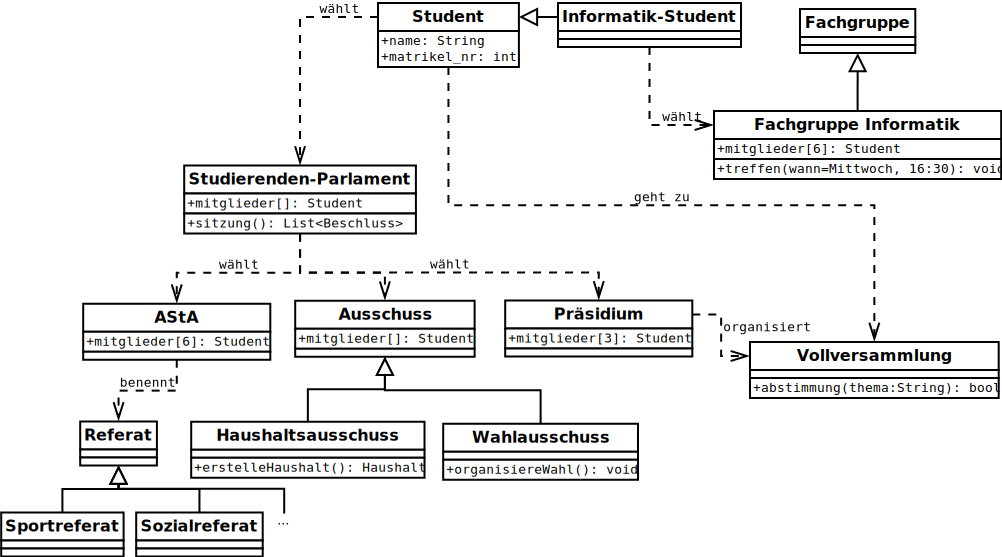
\includegraphics[width=\textwidth]{bilder/gremienkunde2}

		\end{multicols}
		%\begin{multicols}{2}
\subsection{Ich bin unpolitisch!}
	Immer wieder hört man diese Aussage in Vorlesungen, in der Mensa und im Gespräch mit Studierenden beim Fachgruppenrat. Für die meisten Studierenden bedeutet diese Aussage, dass man \emph{kein Interesse an Politik} hat oder zumindest keine Meinung zu aktuellen Vorgängen.

\subsubsection*{Gemäßigtes Braunschweig}

Das Braunschweiger Umfeld macht es einem relativ leicht, sich politisch passiv 
zu verhalten. Hier herrscht nur ein recht kleines Spannungsfeld zwischen den 
traditionell eher rechten studentischen Verbindungen und den traditionell eher 
linken Fachschafts- und Fachgruppenräten sowie dem AStA. Diese 
gegenüberstehenden Parteien werdet ihr in den allermeisten deutschen 
Universitätsstädten wiederfinden. Während es aber anderenorts so richtig 
kracht (Burschenschaftshäuser werden mit Farbbeuteln beworfen und mit Parolen 
beschmiert, jeder öffentliche Auftritt von Burschenschaften führt zu 
Demonstrationen), ist Braunschweig ein gemütliches Pflaster. AStA und die 
Fachschaften finden nur wenige Unterstützer und auch die Burschenschaften 
dominieren in Braunschweig nicht unbedingt das Stadtbild.

\subsubsection*{\emph{Schnell durchziehen!}}

Einen erheblichen Beitrag zur \emph{Ist-mir-doch-egal}-Haltung leistet meiner 
Ansicht nach die heute übliche, ständig über Medien, Politiker oder auch die 
eigenen Eltern verbreitete Doktrin, dass man sein Studium \emph{schnell 
durchziehen}, zielstrebig, leistungs- und ich-orientiert seinen Abschluss 
ansteuern soll. Solche Leute will die Wirtschaft, dafür gibt es Preise und 
Stipendien. Langzeitstudenten werden belächelt und als Sozialfall angesehen. 
Unbequeme Themen wie ethische und religiöse Fragen oder Umweltproblematik 
bleiben bei dieser Sichtweise als erstes auf der Strecke (z.B. gibt es in der 
Informatik in Braunschweig --~anders als zum Beispiel an der Uni Hamburg~-- 
keine Pflichtveranstaltung, die sich mit den gesellschaftlichen Einflüssen der 
Informatik auseinander setzt). Man hat das Gefühl, dass unmündige, 
manipulierbare Arbeitnehmer heranzuzüchtet werden sollen - den früher 
propagierten \emph{breiten Horizont} einer Hochschulausbildung konnte ich an 
unserer TU bisher nicht entdecken.

\subsubsection*{Verbindungen zur Politik}

Nun zurück zum \textbf{weit verbreiteten Gerücht, das eigene Studium habe 
doch nichts mit Politik zu tun}: Die Uni als Institution lässt sich nicht von 
der Politik lösen! Wir sind alle direkt betroffen von der Landespolitik (vor 
allem natürlich Bildungspolitik) und Lokalpolitik (z.B. Radwege, 
Attraktivität der Stadt). Außerdem gibt es auch eine Uni-interne Politik, wie 
euch die \emph{Kleine Gremienkunde} in diesem Heft schon ausführlich dargelegt 
hat. Wer sich z.B. in einem Institut umhört, wird dort nirgends 
Gleichgültigkeit gegenüber der Bildungspolitik zu spüren bekommen. Ob 
Professorenstellen neu besetzt werden, ob genügend HiWis für kleine übungen 
bezahlt werden, ob neue Geräte angeschafft werden, ob gar ganze Studiengänge 
geschlossen werden, ob Studierende bei der Gestaltung ihrer Studiengänge 
mitwirken dürfen, ob öffnungszeiten für bestimmte Dienste verlängert werden 
- all dies hängt von der so viel geschimpften \emph{Politik} der einen oder 
anderen Form ab. \textbf{Politik betrifft euch} und euer Studium. Direkt und 
ohne Wenn und Aber.

Nun will ich natürlich von niemandem verlangen, dass er einer Partei beitritt, 
Straßenaktionen startet oder Bücher schreibt. Aber zumindest ein kleines 
Interesse an eurem direkten Umfeld sollte doch selbstverständlich sein, oder? 
Es hat ja einen Grund, dass euer momentanes Studium so ist, wie es ist. Es gibt 
Studierende, die sich engagieren, die selbst etwas beitragen wollen, z.B. eine 
neue BPO (Bachelorprüfungsordnung) mit erarbeiten, für mehr Computer oder 
längere öffnungszeiten streiten etc., um unseren Studiengang und unser 
Hochschulleben attraktiver zu gestalten.

Übrigens war die Hochschulpolitik bis zum Sommersemester 2011 überwiegend 
unabhängig von parteipolitischen Interessen. Nun sind aber erstmals auch 
Wahllisten angetreten, die etablierten Parteien aus der Landes- und Bundespolitik
nahestehen und dies durch ihren Namen eindeutig aufzeigen. Ob und wie sich dies auf die 
Hochschulpolitik auswirkt, wird sich in den kommenden Semestern zeigen.

\subsubsection*{Informieren und Engagieren}

Wie kann man nun einen Einblick in das, was die Studierenden bewegen und was 
die Studierenden bewegt, gewinnen? Als erstes wären dort die hauptamtlichen 
Mitarbeiter des \textbf{AStA} zu nennen. Hinter der umständlichen Abkürzung 
verbergen sich eine Handvoll Studierende, die entgegen weitläufiger Meinung 
weder Steineschmeißer noch Nazis sondern Studierende wie ihr sind. Dann gibt 
es jeden Monat die \textbf{hochschulöffentliche Sitzung des 
Studierendenparlaments}. Dort tauscht man fächerübergreifend Neuigkeiten aus 
und stimmt über entscheidende Dinge ab, z.B. über die Verwendung der 
studentischen Gelder, den studentischen Haushalt. Mindestens einmal im Semester 
gibt es die sogenannte VV, das ist die \textbf{studentische Vollversammlung} - 
wenn sie beschlussfähig ist, dann ist die Vollversammlung das höchste Gremium 
der Studierenden.
Schließlich finden einmal im Semester die \textbf{studentischen Wahlen} statt 
- da könnt ihr direkt oder indirekt (siehe Gremienkunde) bestimmen, welche 
Studierenden euch in den jeweiligen ämtern vertreten sollen. Aus 
unerfindlichen Gründen ist die Wahlbeteiligung bei den studentischen Wahlen 
stets niedrig. Nehmt das als Aufmunterung -- bei geringer Beteiligung zählt 
eure Stimme um so mehr!
 % redaktionall fragwürdig
		%\subsection[Studiengebühren]{Studiengebühren --\\ eine abschließende
Betrachtung}
\emph{von Henning Günther}

Wir schreiben das Wintersemester 2009/10.
Der Widerstand gegen Studiengebühren liegt in Trümmern.
Nach den vernichtenden Niederlagen im voll\-stän\-di\-gen Boykott der
Studiengebühren im Sommersemster 2007, an dem nur 504 der über 14.000 Studenten teilnahmen und dem darauf folgenden, kaum noch spürbaren ,,5 Euro''-Boykott im Wintersemester 2007/08 sind die Studenten kaum noch zu Widerstand bereit. Im Sommersemster 2008 war das Werk vollbracht, jeder anfängliche Widerstand in alle Winde zerstreut, die anfänglich so breit erscheinende Front der Studiengebührengegner zerschlagen.

Was war geschehen?
Wie konnte sich die vormals so rebellische Studentenschaft, die früher keine Möglichkeit ausließ, gegen das Unrecht zu protestieren, innerhalb von nur einem Jahr in einen in gedemütigter Haltung die Gebühren entrichtenden Haufen Elend verwandeln?

Es hat den Anschein, dass die diabolisch geniale Saat der
Studiengebühren-Fürsprecher, die Daumenschrauben der ,,Campus-Maut'' nicht
sofort und im vollen Umfang anzuziehen, auf ganzer Linie aufgegangen sei. Denn es traf zunächst die, die sich am wenigsten wehren konnten: An Erstsemestern die, da noch nicht eingeschrieben, keinen Boykott wagen
konnten wurde zuerst erprobt, ob 500 Euro ein Preis waren, für den die Studenten zu kämpfen bereit wären. Sie waren es nicht.
Zwar waren viele ,,im Prinzip'' dagegen, taten diese Meinung aber nur mäßig
auf den wenigen Demonstrationen kund.

Die meisten der Studenten scheinen sich inzwischen mit dem Fakt, mit jährlich
1000 Euro weniger auskommen zu müssen, abgefunden zu haben. Kaum jemand gibt sich noch dem Wunschtraum hin, größere Teile der Studenten für irgendeine Form des organisierten Protest zu begeistern.
Es scheint fast als könnten die Studiengebührenschergen bald wieder Morgenluft wittern und in der Lage sein, dank mangelnden Widerstand, ihre kühnsten Träume zu verwirklichen: 1000 Euro Studiengebühren pro Semester und mehr.

Was wird die Zukunft bringen?
Werden die Besiegten weiterhin wie die Gespenster einer längst vergangenen Zeit durch die Unigänge huschen, von einer Vorlesung zur nächsten hetzen, um sich durch ein schnelleres Studium vielleicht ein paar Euro Studiengebühren zu sparen und gelernt haben, stets mit der Angst vor einer Erhöhung der Gebühren zu leben?
Es bleibt zu hoffen dass den Advokaten des Bezahlstudiums dieser Triumph nicht gewährt wird.
%
\end{multicols}
\begin{center}
  \includegraphics[width=\linewidth]{bilder/comics/wondermark003.png}
\end{center}
%
%
\begin{multicols}{2}
	%da momentan keine einhellige meinung vorherrsct erstmal rauslassen
	\newpage
	\section{Sonstiges}
		\label{sonstiges}
		
\subsection{Ansprechpartner}
\paragraph{Fachgruppenrat}
%Zu Beginn des Semesters bietet die Fachgruppe wöchentlich einen Infotermin an - siehe Blog für die konkrete Zeit.

Im Normalfall treffen wir uns jede Woche zum Fachgruppentreffen
%Besprechung. Auch
Den  Termin entnehmt ihr bitte aus
\url{http://fginfo.cs.tu-bs.de/index.php/kontakt/fachgruppe/}.
\\\\
Beide Termine finden im Raum 149/150 des Informatikzentrums statt
(siehe dazu Seite \pageref{campuskarte}), in der vorlesungsfreien Zeit
jedoch nur nach Absprache. 
  Falls du eine Frage hast, kannst du gerne zum regulären
  Fachgruppentreffen kommen, oder einfach so mal vorbei schauen ob
  jemand da ist. Tipp: In der Stunde vor dem Treffen füllt sich der
  Raum schon langsam, also hast du da gute Chancen, Probleme in
  kleinerer Runde zu besprechen. 
 Ansonsten erreicht ihr uns natürlich via
Email unter \url{fginfo@tu-bs.de}.

\paragraph{Fachspezifisches}
Bei Fragen zu einem speziellen Fach auch der jeweilige Professor
bzw. Dozent - keiner von denen beißt! Am besten findet ihr die Profs
über die Seiten der jeweiligen Institute oder die Personensuche unter
\url{http://www.tu-braunschweig.de/suchoptionen/personen}.
%\paragraph{Weitere Ansprechpartner} 
%\begin{itemize}
\paragraph{\small Studiengangskoordinatorin} \ \\ Yvonne Sehnert ist die Studiengangskoordinatorin. Sie steht extra bereit,
um euch Fragen zu beantworten, und für alles, was sie nicht selbst
weiß, weiß sie, an wen Sie eure Frage weiterleiten muss.\\
{
Yvonne Sehnert\\
Carl-Friedrich-Gauß-Fakultät\\
Rebenring 58 A | Raum 124\\
Sprechzeiten: Nach  Vereinbarung\\
Telefon: (0531) 391-2843\\
E-Mail: \url{informatik-studium@tu-bs.de}
}

% \paragraph{\small Informatik Service-Desk}
% Heidi Schulze\\
% Informatikzentrum\\
% Mühlenpfordtstraße 23 | Raum G53\\
% Telefon: (0531)391-2116\\
% E-Mail: \url{schulze@cg.cs.tu-bs.de}\\
% \\
% Sprechzeiten: \\
% Mo. 10:00-12:00 Uhr
% \& 13:00-14:30 Uhr
% \\
% Do. 9:00-12:00 Uhr
% \& 13:00-16:30 Uhr
% %\end{itemize}
%\ \ \ \ \\ \\ \\ \\ \ \\
\paragraph{\small{Fachstudienberater}} \ \\
Dr. Werner Struckmann\\
Institut für Programmierung und Reaktive Systeme\\
Mühlenpfordtstraße 23 | Raum 244\\
Telefon: (0531) 391-3278\\
E-Mail: \url{struck@ips.cs.tu-bs.de}\\
\\
Sprechzeiten: Mi. 10:30-11:30 Uhr und nach  Vereinbarung

\paragraph{\small{Prüfungsamt}} \ \\
Rebecca Weidner\\
Carl-Friedrich-Gauß-Fakultät\\
Rebenring 58 A | Raum 127\\
Tel.: (0531) 391-2844\\
Fax: (0531) 391-8225\\
E-Mail: \url{pa-informatik@tu-braunschweig.de}\\
\\
Sprechzeit im Semester:\\
Di. und Do.:
9:30–12:00 Uhr und 14:00-16:30 Uhr\\
\\
Sprechzeit in der vorlesungsfreien Zeit:\\
Di. und Do.
9:30-12:00 Uhr \\


% Local Variables: 
% mode: latex
% TeX-master: "../../1-te"
% End: 

		\subsection{Lernräume}
	Hier wollen wir euch eine aktuelle Übersicht über Lernräume an der TU Braunschweig geben. Die Liste ist im Moment nicht vollständig, sie wird aber demnächst erweitert und ist dann auf \url{http://fginfo.cs.tu-bs.de/index.php/studium/lernraume/} zu finden. Alle Gebäude stehen, wenn nicht anders in Anlage 1 der Hausordnung der TU Braunschweig erwähnt, von 7:30 bis 19:30 Uhr offen.
	\subsubsection*{Informatikzentrum}
		\begin{tabular}{|p{4cm}|p{4cm}|p{8cm}|}
			\hline Raum & Öffnungszeiten & Ausstattung \\ 
			\hline Plaza des Informatikzentrums & normal &  Tische und Stühle, Steckdosen unter Bodenabdeckungen zu finden \\
			\hline Fachgruppenraum der Informatik IZ 150 &
			nach Absprache mit Mitgliedern des
			Fachgruppenrates (wir ;) ) & Kaffemaschine, Sofas, Tische, Steckdosen in Massen sowie Ethernetkabel\\ 
			\hline Fachgruppenraum der Wirtschaftsinformatik
			IZ 159 & nach Absprache mit Mitgliedern des
			Fachgruppenrates Wirtschaftsinformatik (unsere
			netten Nachbarn :) )& Sofas, Tische und Steckdosen \\ 
			\hline CIP Pool IZ G40 & normal & Rechner-Pool mit Linux-PCs, Tafel\\ 
			\hline Gruppenarbeitsraum IZ 033 & normal &
			solange nicht anders belegt, Schlüssel gegen
			Pfand im Sekeratrat der Robotik bei Frau Engel,
			Raum G13 erhältlich.
			\hline
		\end{tabular}
	\subsubsection*{Andere Lernräume}
		\begin{tabular}{|p{4cm}|p{4cm}|p{3.6cm}|p{4cm}|}
 			\hline Raum & Öffnungszeiten & Ausstattung & Anmerkung  \\  
			\hline Grotrian  Zimmerstraße 24 & Normal  & Alte Tische und Stühle, vereinzelt Tafeln & Wenn Mitglieder der verschiedenen Fachgruppen anwesend sind hat das Grotrian meist länger offen. Da dies oft der Fall ist kann man hier meist lange lernen. \\ 
			\hline Bibliothek & Mo - Fr: 07:00 - 24:00 Sa: 10:00 - 20:00& Niedrige Tische und Stühle, Ruhezone, Rechnerarbeits\-plätze, Kopierer &  nicht zum  Lernen in der Gruppe  geeignet \\ 
			\hline Mensa / Cafeteria & Mo -Do: 08 - 20:00 Uhr Fr: 08:00 - 15:00 & Tische, Stühle, kein (!) WLAN, einzelner Rechner mit Netzzugang, Verpflegung incl. Selbstbedienungs-Kaffeeautomat& Probleme: Nicht durchgehend geöffnet, die Plätze sind primär zu Essen gedacht, von Lernsessions zu den Stoßzeiten sollte man also im eigenen und fremden Interesse absehen. \\ 
			\hline Bei dir zuhause & immer & Deine Sache & Achtung: Man lenkt sich leicht ab :) \\ 
			\hline Das eine oder andere Cafe / Kneipe & kommt drauf an & wechselhaft &Siehe die beiden vorherigen \\
			\hline
		\end{tabular}

		% rausgenommen, da scheiße zu lesen und an anderer
		% stelle dokumentiert (jst)

		%\begin{multicols}{2}
\subsection{Semesterticket}
	Euer Studentenausweis berechtigt euch zur Fahrt auf vielen Zugstrecken in Niedersachsen. Unten seht ihr den Gültigkeitsbereich des Semestertickets im Großraum Hannover. Nach Norden und und Westen deckt das Semesterticket weitere Strecken ab. Einen grober Überblick gibt die nebenstehende Karte. 

	Es d"urfen nur Regionalexpress (RE) und Regionalbahn (RB) der Deutschen Bahn AG, sowie teilweise der Metronom in der zweiten Klasse benutzt werden. Also NICHT Strecken der Nordwestbahn (NWB). Einen genauen Überblick findet ihr in Form einer Streckenliste auf der Seite \pageref{streckenliste1}.

	Mehr Details könnt ihr den Seiten des AStA unter \url{http://www.asta.tu-bs.de/semesterticket.php} bzw. \url{http://tinyurl.com/3gn8fhg} entnehmen.
\end{multicols}
\newpage
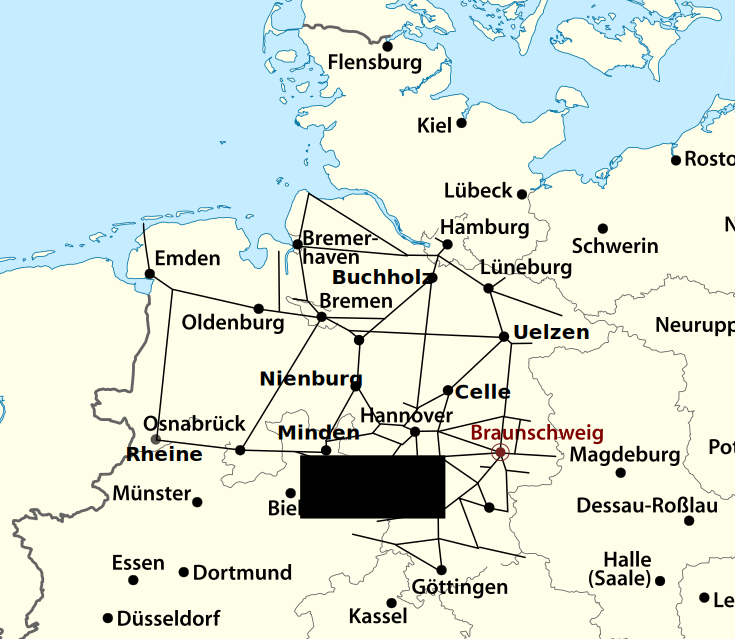
\includegraphics[width=\columnwidth]{bilder/ticket_deutschland.png}
\newpage
\includegraphics[width=\textwidth]{bilder/ticket_bis_11_Dezember.jpg}
\newpage
%\newpage
%\begin{table}[htbp]
Streckenübersicht Wintersemester 2010/2011 und Sommersemester 2011 gültig ab 1.10.2010

\enlargethispage{0.5cm} 
 
%  \begin{addmargin}{-1.5cm}
%\begin{center}
\begin{tabular}{|l|l|l|p{2cm}|}
\hline
\multicolumn{3}{|l|}{\textbf{Strecke/ Streckenabschnitt}}& \textbf{KbN}\\
\textbf{\textit{von}} & \textit{über} & \textbf{\textit{bis}} & \\ \cline{ 1- 4}
Lüneburg &  & Dannenberg Ost & 112 \\ \hline
Braunschweig Hbf & Gifhorn & Uelzen & 115 \\ \hline
Bremen Hbf & Soltau & Uelzen & 116 \\ \hline
Hamburg-Harburg &  & Stade & 121 \\ \hline
Buchholz (Nordheide) & Soltau & Bennemühlen & 123 \\ \hline
Minden Westf. & Nienburg & Rotenburg/Bremen Hbf & 124 \\ \hline
Bremen Hbf &  & Cuxhaven & 125 \footnotemark[1] \\ \hline
Bremen Hbf &  & Bremen-Vegesack & 126 \footnotemark[1] \\ \hline
Echem &  & Lüneburg & 145 \\ \hline
Hannover Hbf & Gifhorn & Wolfsburg Hbf & 300 \\ \hline
Braunschweig Hbf &  & Wolfsburg Hbf & 301 \\ \hline
Uelzen &  & Schnega & 305 \\ \hline
Hannover Hbf & Braunschweig Hbf & Helmstedt & 310 \\ \hline
Braunschweig Hbf & Wolfenbüttel & Schöppenstedt & 312 \footnotemark[2] \\ \hline
Braunschweig Hbf &  & Hildesheim Hbf & 313 \\ \hline
Hannover Hbf & Hildesheim Hbf/Goslar & Bad Harzburg & 320 \\ \hline
Braunschweig Hbf &  & Sz-Lebenstedt & 352 \\ \hline
Braunschweig Hbf & Wolfenbüttel/Vienenburg & Goslar & 353 \\ \hline
Holzminden & Kreiensen & Bad Harzburg & 354 \\ \hline
Ottbergen & Bodenfelde & Göttingen & 356.1 \\ \hline
Ottbergen & Bodenfelde & Northeim & 356.2 \\ \hline
Göttingen & Northeim & Walkenried & 357 \footnotemark[1] \\ \hline
Braunschweig Hbf & Seesen & Herzberg (Harz) & 358 \\ \hline
Haste & Hannover Hbf/Haste & Minden (Westf) & 360.1 \\ \hline
Nienburg (Weser) & Hannover Hbf & Haste & 360.2 \\ \hline
Hannover Hbf & Lehrte & Hildesheim Hbf & 360.3 \\ \hline
Bennemühlen & Hann./Sarstedt & Hildesheim Hbf & 360.4 \\ \hline
Bad Pyrmont & Hameln/Weetzen & Hannover-Flughafen & 360.5 \\ \hline
Celle & Lehrte & Hannover Hbf & 360.6.7 \\ \hline
Hannover Hbf &  & Hannover Bismarckstr. & 361 \footnotemark[1] \\ \hline
Hannover Hbf &  & Löhne (Westf.) & 370 \\ \hline
Löhne (Westf.) & Hameln & Hildesheim Hbf & 372 \\ \hline
Hildesheim Hbf &  & Bodenburg & 373 \\ \hline
Salzbergen & Osnabrück Hbf & Minden (Westf.) & 375 \footnotemark[1] \\ \hline
Bremen Hbf &  & Hannover Hbf & 380 \\ \hline
Osnabrück Hbf &  & Bremen Hbf & 385 \footnotemark[1] \\ \hline
Norddeich Mole & Oldenburg (Oldb) & Bremen Hbf & 390 \footnotemark[1] \\ \hline
Norddeich Mole & Meppen & Rheine & 395 \footnotemark[1] \\ \hline
Emden Hbf &  & Emden Außenhafen & 396 \\ \hline
Leer (Ostfr.) &  & Weener & 397 \\ \hline
\end{tabular}

\footnotetext[1]{nur in den Zügen der DB Regio AG, also nicht in Zügen der Nordwestbahn}
\footnotetext[2]{gültig auch in Bus von  Schöppenstedt-Schöningen-Helmstedt}
%\end{tabular}
%  \end{addmargin}
\label{streckenliste1}
%\end{table}
%\begin{table}[htbp]

%\newpage
%Streckenübersicht Wintersemester 2010 gültig bis 11.12.2010
%
%  \begin{addmargin}{-1.5cm}
%\begin{tabular}{|l|l|l|p{1cm}|}
%\hline
%\multicolumn{3}{|l|}{\textbf{Strecke/ Streckenabschnitt}}& \textbf{KbN}\\
%\textbf{\textit{von}} & \textit{über} & \textbf{\textit{bis}} & \\ \cline{ 1- 4}
%Lüneburg &  & Dannenberg Ost & 112 \\ \hline
%Braunschweig Hbf & Gifhorn & Uelzen & 115 \\ \hline
%Bremen Hbf & Soltau & Uelzen & 116 \\ \hline
%Bremen Hbf &  & Rotenburg/W. & 120 * / *** \\ \hline
%Hamburg-Harburg &  & Stade & 121 \\ \hline
%Buchholz (Nordheide) & Soltau & Bennemühlen & 123 \\ \hline
%Minden Westf. & Nienburg & Rotenburg/Bremen Hbf   & 124 \\ \hline
%Bremen Hbf &  & Cuxhaven & 125 \\ \hline
%Bremen Hbf &  & Bremen-Vegesack & 126* \\ \hline
%Echem &  & Lüneburg & 145 \\ \hline
%Hannover Hbf & Gifhorn & Wolfsburg Hbf & 300 \\ \hline
%Braunschweig Hbf &  & Wolfsburg Hbf & 301 \\ \hline
%Uelzen &  & Schnega & 305 \\ \hline
%Hannover Hbf & Braunschweig Hbf & Helmstedt & 310 \\ \hline
%Braunschweig Hbf & Wolfenbüttel & Schöppenstedt & 312 ** \\ \hline
%Braunschweig Hbf &  & Hildesheim Hbf & 313 \\ \hline
%Hannover Hbf & Hildesheim Hbf/Goslar & Bad Harzburg & 320 \\ \hline
%Braunschweig Hbf &  & Sz-Lebenstedt & 352 \\ \hline
%Braunschweig Hbf & Wolfenbüttel/Vienenburg & Goslar & 353 \\ \hline
%Holzminden & Kreiensen & Bad Harzburg & 354 \\ \hline
%Ottbergen & Bodenfelde & Göttingen & 356.1 \\ \hline
%Ottbergen & Bodenfelde & Northeim & 356.2 \\ \hline
%Göttingen & Northeim & Walkenried & 357 * \\ \hline
%Braunschweig Hbf & Seesen & Herzberg (Harz) & 358 \\ \hline
%Haste & Hannover Hbf/Haste & Minden (Westf) & 360.1 \\ \hline
%Nienburg/Weser & Hannover Hbf & Haste (Han) & 360.2 \\ \hline
%Hannover Hbf & Lehrte & Hildesheim Hbf & 360.3 \\ \hline
%Bennemühlen & Hann./Sarstedt & Hildesheim Hbf & 360.4 \\ \hline
%Bad Pyrmont & Hameln/Weetzen & Hannover-Flughafen & 360.5 \\ \hline
%Celle & Lehrte & Hannover Hbf & 360.6.7 \\ \hline
%Hannover Hbf &  & Hannover Bismarckstr. & 361 * \\ \hline
%Hannover Hbf &  & Löhne (Westf.) & 370 \\ \hline
%Löhne (Westf.) & Hameln & Hildesheim Hbf & 372 \\ \hline
%Hildesheim Hbf &  & Bodenburg & 373 \\ \hline
%Salzbergen & Osnabrück Hbf & Minden (Westf.) & 375 * \\ \hline
%Bremen Hbf &  & Hannover Hbf & 380 \\ \hline
%Osnabrück Hbf &  & Bremen Hbf & 385 \\ \hline
%Norddeich Mole & Oldenburg (Oldb) & Bremen Hbf & 390 * \\ \hline
%Nordenham &  & Bremen Hbf & 391 \\ \hline
%Norddeich Mole & Meppen & Rheine & 395 \\ \hline
%Emden Hbf &  & Emden Außenhafen                     & 396 \\ \hline
%Leer (Ostfr.) &  & Weener & 397 \\ \hline
%\end{tabular}
%\enlargethispage{1cm}
%
%\textbf{* nur in den Zügen der DB Regio AG ** gültig auch in Bus von
%  Schöppenstedt-Schöningen-Helmstedt KbN Kursbuch-Nr}
%\end{tabular}
%  \end{addmargin}
%\label{streckenliste2}
%\end{table}

% Local Variables: 
% mode: latex
% TeX-master: "../../1-te"
% End: 

	      %\end{multicols}
		\newpage
\subsection{Impressum}
\label{impressum}
\begin{description}
\item[Herausgeber:]
	Fachgruppe Informatik\\
	c/o AStA der TU Braunschweig\\
	Katharinenstraße 1\\
	38106 Braunschweig\\
	Tel.: 0531/391-4569\\
	E-Mail: \url{fginfo@tu-bs.de}\\
	Webseite: \url{http://fginfo.cs.tu-bs.de/}
\item[V.i.S.d.P.:]  % Verantwortliche(r) im Sinne des Presserechts
  Lena Schimmel, Johannes Starosta
\end{description}
\end{document}
